%==============================================================================
% tento soubor pouzijte jako zaklad
% this file should be used as a base for the thesis
% Autoři / Authors: 2008 Michal Bidlo, 2019 Jaroslav Dytrych
% Kontakt pro dotazy a připomínky: sablona@fit.vutbr.cz
% Contact for questions and comments: sablona@fit.vutbr.cz
%==============================================================================
% kodovani: UTF-8 (zmena prikazem iconv, recode nebo cstocs)
% encoding: UTF-8 (you can change it by command iconv, recode or cstocs)
%------------------------------------------------------------------------------
% zpracování / processing: make, make pdf, make clean
%==============================================================================
% Soubory, které je nutné upravit nebo smazat: / Files which have to be edited or deleted:
%   projekt-20-literatura-bibliography.bib - literatura / bibliography
%   projekt-01-kapitoly-chapters.tex - obsah práce / the thesis content
%   projekt-01-kapitoly-chapters-en.tex - obsah práce v angličtině / the thesis content in English
%   projekt-30-prilohy-appendices.tex - přílohy / appendices
%   projekt-30-prilohy-appendices-en.tex - přílohy v angličtině / appendices in English
%==============================================================================
%\documentclass[]{fitthesis} % bez zadání - pro začátek práce, aby nebyl problém s překladem
%\documentclass[english]{fitthesis} % without assignment - for the work start to avoid compilation problem
\documentclass[zadani,slovak]{fitthesis} % odevzdani do wisu a/nebo tisk s barevnými odkazy - odkazy jsou barevné
%\documentclass[english,zadani]{fitthesis} % for submission to the IS FIT and/or print with color links - links are color
%\documentclass[zadani,print]{fitthesis} % pro černobílý tisk - odkazy jsou černé
%\documentclass[english,zadani,print]{fitthesis} % for the black and white print - links are black
%\documentclass[zadani,cprint]{fitthesis} % pro barevný tisk - odkazy jsou černé, znak VUT barevný
%\documentclass[english,zadani,cprint]{fitthesis} % for the print - links are black, logo is color
% * Je-li práce psaná v anglickém jazyce, je zapotřebí u třídy použít 
%   parametr english následovně:
%   If thesis is written in English, it is necessary to use 
%   parameter english as follows:
%      \documentclass[english]{fitthesis}
% * Je-li práce psaná ve slovenském jazyce, je zapotřebí u třídy použít 
%   parametr slovak následovně:
%   If the work is written in the Slovak language, it is necessary 
%   to use parameter slovak as follows:
%      \documentclass[slovak]{fitthesis}
% * Je-li práce psaná v anglickém jazyce se slovenským abstraktem apod., 
%   je zapotřebí u třídy použít parametry english a enslovak následovně:
%   If the work is written in English with the Slovak abstract, etc., 
%   it is necessary to use parameters english and enslovak as follows:
%      \documentclass[english,enslovak]{fitthesis}

% Základní balíčky jsou dole v souboru šablony fitthesis.cls
% Basic packages are at the bottom of template file fitthesis.cls
% zde můžeme vložit vlastní balíčky / you can place own packages here

% Kompilace po částech (rychlejší, ale v náhledu nemusí být vše aktuální)
% Compilation piecewise (faster, but not all parts in preview will be up-to-date)
% \usepackage{subfiles}

% Nastavení cesty k obrázkům
% Setting of a path to the pictures
%\graphicspath{{obrazky-figures/}{./obrazky-figures/}}
%\graphicspath{{obrazky-figures/}{../obrazky-figures/}}

%---rm---------------
\renewcommand{\rmdefault}{lmr}%zavede Latin Modern Roman jako rm / set Latin Modern Roman as rm
%---sf---------------
\renewcommand{\sfdefault}{qhv}%zavede TeX Gyre Heros jako sf
%---tt------------
\renewcommand{\ttdefault}{lmtt}% zavede Latin Modern tt jako tt

% vypne funkci šablony, která automaticky nahrazuje uvozovky,
% aby nebyly prováděny nevhodné náhrady v popisech API apod.
% disables function of the template which replaces quotation marks
% to avoid unnecessary replacements in the API descriptions etc.
\csdoublequotesoff



\usepackage{url}
\usepackage{svg}
\usepackage{caption}
\usepackage{subcaption}


% =======================================================================
% balíček "hyperref" vytváří klikací odkazy v pdf, pokud tedy použijeme pdflatex
% problém je, že balíček hyperref musí být uveden jako poslední, takže nemůže
% být v šabloně
% "hyperref" package create clickable links in pdf if you are using pdflatex.
% Problem is that this package have to be introduced as the last one so it 
% can not be placed in the template file.
\ifWis
\ifx\pdfoutput\undefined % nejedeme pod pdflatexem / we are not using pdflatex
\else
  \usepackage{color}
  \usepackage[unicode,colorlinks,hyperindex,plainpages=false,pdftex]{hyperref}
  \definecolor{hrcolor-ref}{RGB}{223,52,30}
  \definecolor{hrcolor-cite}{HTML}{2F8F00}
  \definecolor{hrcolor-urls}{HTML}{092EAB}
  \hypersetup{
	linkcolor=hrcolor-ref,
	citecolor=hrcolor-cite,
	filecolor=magenta,
	urlcolor=hrcolor-urls
  }
  \def\pdfBorderAttrs{/Border [0 0 0] }  % bez okrajů kolem odkazů / without margins around links
  \pdfcompresslevel=9
\fi
\else % pro tisk budou odkazy, na které se dá klikat, černé / for the print clickable links will be black
\ifx\pdfoutput\undefined % nejedeme pod pdflatexem / we are not using pdflatex
\else
  \usepackage{color}
  \usepackage[unicode,colorlinks,hyperindex,plainpages=false,pdftex,urlcolor=black,linkcolor=black,citecolor=black]{hyperref}
  \definecolor{links}{rgb}{0,0,0}
  \definecolor{anchors}{rgb}{0,0,0}
  \def\AnchorColor{anchors}
  \def\LinkColor{links}
  \def\pdfBorderAttrs{/Border [0 0 0] } % bez okrajů kolem odkazů / without margins around links
  \pdfcompresslevel=9
\fi
\fi
% Řešení problému, kdy klikací odkazy na obrázky vedou za obrázek
% This solves the problems with links which leads after the picture
\usepackage[all]{hypcap}

% Informace o práci/projektu / Information about the thesis
%---------------------------------------------------------------------------
\projectinfo{
  %Prace / Thesis
  project={BP},            %typ práce BP/SP/DP/DR  / thesis type (SP = term project)
  year={2022},             % rok odevzdání / year of submission
  date=\today,             % datum odevzdání / submission date
  %Nazev prace / thesis title
  title.cs={Systém pro chytrou regulaci ústředního topení},  % název práce v češtině či slovenštině (dle zadání) / thesis title in czech language (according to assignment)
  title.en={System for Smart Central Heating Regulation}, % název práce v angličtině / thesis title in english
  title.length={14.5cm}, % nastavení délky bloku s titulkem pro úpravu zalomení řádku (lze definovat zde nebo níže) / setting the length of a block with a thesis title for adjusting a line break (can be defined here or below)
  %sectitle.length={14.5cm}, % nastavení délky bloku s druhým titulkem pro úpravu zalomení řádku (lze definovat zde nebo níže) / setting the length of a block with a second thesis title for adjusting a line break (can be defined here or below)
  %dectitle.length={14.5cm}, % nastavení délky bloku s titulkem nad prohlášením pro úpravu zalomení řádku (lze definovat zde nebo níže) / setting the length of a block with a thesis title above declaration for adjusting a line break (can be defined here or below)
  %Autor / Author
  author.name={Jakub},   % jméno autora / author name
  author.surname={Sikula},   % příjmení autora / author surname 
  %author.title.p={Bc.}, % titul před jménem (nepovinné) / title before the name (optional)
  %author.title.a={Ph.D.}, % titul za jménem (nepovinné) / title after the name (optional)
  %Ustav / Department
  department={UIFS}, % doplňte příslušnou zkratku dle ústavu na zadání: UPSY/UIFS/UITS/UPGM / fill in appropriate abbreviation of the department according to assignment: UPSY/UIFS/UITS/UPGM
  % Školitel / supervisor
  supervisor.name={Jiří},   % jméno školitele / supervisor name 
  supervisor.surname={Hynek},   % příjmení školitele / supervisor surname
  supervisor.title.p={Ing.},   %titul před jménem (nepovinné) / title before the name (optional)
  supervisor.title.a={Ph.D.},    %titul za jménem (nepovinné) / title after the name (optional)
  % Klíčová slova / keywords
  keywords.cs={Kúrenie, Regulácia kúrenia, Smart Home, Smart kúrenie, IOT, LoRaWan, Typescript, LNS, Logimic, iTemp.}, % klíčová slova v českém či slovenském jazyce / keywords in czech or slovak language
  keywords.en={Heating, Heating regulation, Smart Home, Smart heating, IOT, LoRaWan, Typescript, LNS, Logimic, iTemp.}, % klíčová slova v anglickém jazyce / keywords in english
  %keywords.en={Here, individual keywords separated by commas will be written in English.},
  % Abstrakt / Abstract
  abstract.cs={Cieľom tejto bakalárskej práce bolo navrhnúť a implementovať systém regulácie ústredného kúrenia so zameraním na reguláciu jednotlivých miestností. 
  Tento systém je diaľkovo ovládateľný platformou Logimic Smart City a automaticky regulouje vytápanie adaptívnym spôsobom. 
  Tento spôsob prináša značné úspory do domácností, ktoré sú takýmto systémom vybavené. 
  Toto riešenie sa oproti existujúcim riešeniam líšiť hlavne tým, že si do systému zadáme požadovanú teplotu miestnosti a systém ovláda výhrevné telesá tak, aby požadovanú teplotu miestnosti docielili a udržali.}, % abstrakt v českém či slovenském jazyce / abstract in czech or slovak language
  abstract.en={The goal of this bachelor's thesis was to design and implement a central heating control system with a focus on the control of individual rooms. This system is remotely controlled by the Logimic Smart City platform and automatically regulates the heating in an adaptive way. This method brings significant savings to households that are equipped with such a system. This solution differs from existing solutions mainly in that we enter the desired room temperature into the system and the system controls the heating elements so that they reach and maintain the desired room temperature.}, % abstrakt v anglickém jazyce / abstract in english
  %abstract.en={An abstract of the work in English will be written in this paragraph.},
  % Prohlášení (u anglicky psané práce anglicky, u slovensky psané práce slovensky) / Declaration (for thesis in english should be in english)
  declaration={Prehlasujem, že som túto bakalársku prácu vypracoval samostatne pod vedením pana Ing.~Jiřího Hynka, Ph.D.
Dalšie informácie mi poskytli Ing. Michal Valný a Ing. František Mikulu, vývojari firmy Logimic a Ing. Slavomír Satvár z firmy Virtuálny správca budov. 
Uviedol som všetky literárne pramene, publikacie a dalšie zdroje, z ktorých som čerpal.},
  %declaration={I hereby declare that this Bachelor's thesis was prepared as an original work by the author under the supervision of Mr. X
% The supplementary information was provided by Mr. Y
% I have listed all the literary sources, publications and other sources, which were used during the preparation of this thesis.},
  % Poděkování (nepovinné, nejlépe v jazyce práce) / Acknowledgement (optional, ideally in the language of the thesis)
  acknowledgment={Týmto by som chcel poďakovať Ing. Jiřímu Hynkovi, Ph.D, za odborné vedenie mojej práce, konzultácie, rady a hlavne trpezlivosť a ochotu. Ďalej by som chcel poďakovať vývojárom firmy Logimic Ing. Michalovi Valnému a Ing. Františkovi Mikulu za poskytnutie zariadení a ďalších prostriedkov pre vývoj, ako aj cenných rád pri implementácii. V neposlednej rade, by som chcel poďakovať Ing. Slavomírovi Satvárovi za rozhovor a poskytnuté informácie, rovnako ako aj všetkým anonymným respodentom.},
  %acknowledgment={Here it is possible to express thanks to the supervisor and to the people which provided professional help
%(external submitter, consultant, etc.).},
  % Rozšířený abstrakt (cca 3 normostrany) - lze definovat zde nebo níže / Extended abstract (approximately 3 standard pages) - can be defined here or below
  %extendedabstract={Do tohoto odstavce bude zapsán rozšířený výtah (abstrakt) práce v českém (slovenském) jazyce.},
  %extabstract.odd={true}, % Začít rozšířený abstrakt na liché stránce? / Should extended abstract start on the odd page?
  %faculty={FIT}, % FIT/FEKT/FSI/FA/FCH/FP/FAST/FAVU/USI/DEF
  faculty.cs={Fakulta informačních technologií}, % Fakulta v češtině - pro využití této položky výše zvolte fakultu DEF / Faculty in Czech - for use of this entry select DEF above
  faculty.en={Faculty of Information Technology}, % Fakulta v angličtině - pro využití této položky výše zvolte fakultu DEF / Faculty in English - for use of this entry select DEF above
  department.cs={Ústav matematiky}, % Ústav v češtině - pro využití této položky výše zvolte ústav DEF nebo jej zakomentujte / Department in Czech - for use of this entry select DEF above or comment it out
  department.en={Institute of Mathematics} % Ústav v angličtině - pro využití této položky výše zvolte ústav DEF nebo jej zakomentujte / Department in English - for use of this entry select DEF above or comment it out
}

% Rozšířený abstrakt (cca 3 normostrany) - lze definovat zde nebo výše / Extended abstract (approximately 3 standard pages) - can be defined here or above
%\extendedabstract{Do tohoto odstavce bude zapsán výtah (abstrakt) práce v českém (slovenském) jazyce.}
% Začít rozšířený abstrakt na liché stránce? / Should extended abstract start on the odd page?
%\extabstractodd{true}

% nastavení délky bloku s titulkem pro úpravu zalomení řádku - lze definovat zde nebo výše / setting the length of a block with a thesis title for adjusting a line break - can be defined here or above
%\titlelength{14.5cm}
% nastavení délky bloku s druhým titulkem pro úpravu zalomení řádku - lze definovat zde nebo výše / setting the length of a block with a second thesis title for adjusting a line break - can be defined here or above
%\sectitlelength{14.5cm}
% nastavení délky bloku s titulkem nad prohlášením pro úpravu zalomení řádku - lze definovat zde nebo výše / setting the length of a block with a thesis title above declaration for adjusting a line break - can be defined here or above
%\dectitlelength{14.5cm}

% řeší první/poslední řádek odstavce na předchozí/následující stránce
% solves first/last row of the paragraph on the previous/next page
\clubpenalty=10000
\widowpenalty=10000

% checklist
\newlist{checklist}{itemize}{1}
\setlist[checklist]{label=$\square$}

% Nechcete-li, aby se u oboustranného tisku roztahovaly mezery pro zaplnění stránky, odkomentujte následující řádek / If you do not want enlarged spacing for filling of the pages in case of duplex printing, uncomment the following line
% \raggedbottom

\begin{document}
  % Vysazeni titulnich stran / Typesetting of the title pages
  % ----------------------------------------------
  \maketitle
  % Obsah
  % ----------------------------------------------
  \setlength{\parskip}{0pt}
    
  {\hypersetup{hidelinks}\setcounter{tocdepth}{1}\tableofcontents}
  
  % Seznam obrazku a tabulek (pokud prace obsahuje velke mnozstvi obrazku, tak se to hodi)
  % List of figures and list of tables (if the thesis contains a lot of pictures, it is good)
  \ifczech
    \renewcommand\listfigurename{Seznam obrázků}
  \fi
  \ifslovak
    \renewcommand\listfigurename{Zoznam obrázkov}
  \fi
  % {\hypersetup{hidelinks}\listoffigures}
  
  \ifczech
    \renewcommand\listtablename{Seznam tabulek}
  \fi
  \ifslovak
    \renewcommand\listtablename{Zoznam tabuliek}
  \fi
  % {\hypersetup{hidelinks}\listoftables}

  \ifODSAZ
    \setlength{\parskip}{0.5\bigskipamount}
  \else
    \setlength{\parskip}{0pt}
  \fi

  % vynechani stranky v oboustrannem rezimu
  % Skip the page in the two-sided mode
  \iftwoside
    \cleardoublepage
  \fi

  % Text prace / Thesis text
  % ----------------------------------------------
  %\ifenglish
  %  \input{projekt-01-kapitoly-chapters-en}
  %\else
  %  \input{projekt-01-kapitoly-chapters}
  %\fi
  
  \setcounter{secnumdepth}{3}
  \chapter{Úvod}
Každý človek ku komfortnému životu potrebuje pre neho komfortnú teplotu. 
To dosahujú zapaľovaním ohňov, prikladajú do piecok alebo napríklad ženú horúcu vodu radiátorom, aby zmiernili efekty vonkajšej zimy a vytvorili si tepelnú pohodu. 
Od ohniska v~jaskyni, ľudia vo vykurovaní urobili riadny pokrok. 
Technologický vývoj v~oblasti internetu vecí ponúka možnosť aplikovať tieto nové bezdrátové technológie aj na túto sféru života~a~bývania. 
A~to tak, že pripojíme aj kúrenie k~internetu s~cieľom využiť jeho sily pre uľahčenie prístupu ku regulácii a hlavne ušetrenia nákladov na kúrenie. 

Cieľom je návrhnúť a implementovať inteligentný systém pre reguláciu ústredného kúrenia. 
Hlavnou úlohou systému je inteligentná časť, ktorá ovláda výhrevné telesá v~miestnostiach za účelom dosiahnutia ideálnej teploty miestnosti~a~jej udržiavanie. 
Druhá časť je ponúknuť užívateľom diaľkový, prehľadný~a~intuitívny spôsob ovládania tohto systému. 
Celkovým výstupom mala byť aplikácia prístupná z~platformy ACADA aplikácie iTemp firmy Logimic. 
Táto aplikácia mala priniesť jednoduchý diaľkový spôsob ovládania teploty v~miestnosti vybavenej tepelnými senzormi a ovládateľnou výhrevnou jednotkou.

Táto práca je logicky rozdelená do niekoľkých oddelených kapitol a podkapitol. 
Úvodné kapitoly sa zameriavajú na teóriu ohľadom technológii a to hlavne na sféru internetu vecí v kapitole \ref{Internet_veci}, nakoľko táto téma spadá do tejto kategórie. 
Ďalej pokračuje rozsiahla téma problematiky kúrenia v kapitole \ref{kur}, ktorá vysvetľuje základné pojmy ohľadom kúrenia, spôsoby ovládania a problémy, ktoré ho sprevádzajú. 
Ďalej sú v kapitole \ref{anal} analyzované požiadavky na systém, jeho užívateľov a existujúce riešenia. 
Na základe výsledku analýzy je v~ďalšej kapitole \ref{navrh} návrh systému. 
Ten sa venuje architektúre systému, datovému modelu, algoritmu inteligentného kúrenia a ďalším částiam.
Kapitola \ref{impl} sa venuje popisu implementácie návrhu. 
Konkrétne sa venuje použitým zariadeniam, LoRa serveru, obsluhe zariadení a aplikácii iTemp. 
Predposledná kapitola \ref{test} sa venuje testovaniu vytvoreného systému. 
To je rozdelené do dvoch části na testovanie v simulácii s fiktívnymi datami a testovanie v reálnom prostredí.
Posledná kapitola \ref{zaver} zhodnocuje celú prácu.
  \chapter{Internet vecí}\label{Internet_veci}
Bakalárska práca je založená na myšlienke a technológiách \emph{internetu vecí}, preto je mu venovaná táto kapitola. 
V~podkapitole \ref{iot-history} je obsiahnutá krátka história \emph{internetu vecí} (ďalej už len skratka IoT z~anglického \emph{internet of things}), definícia čo IoT v~dnešnej dobe predstavuje je v~podkapitole \ref{iot-definition} a podkapitola \ref{iot-smartcity} sa venuje IoT v~rozsahu celých miest. 
V~podkapitole \ref{Iot-technology} sú zhrnuté základné technológie používané v~IoT.

\section{História}\label{iot-history}
Napriek pár zariadeniam, ktoré boli už skôr pripojené na internet, bolo pravdepodobne IoT prvýkrát spomenuté iba ako názov prezentácie z~roku 1999, ktorej autorom bol Kevin Ashton~\cite{ashton2009internet}. 
V~tom čase boli takmer všetky dáta na internete vytvorené a nahraté ľuďmi. 
Jeho myšlienkou bolo zapojiť do internetu nielen ľudí ale aj predmety. 
Tie mali byť schopné komunikovať a zdieľať  o~sebe informácie bez ľudskej interakcie. 
Tým chcel dosiahnuť, aby sme mohli všetko sledovať, spočítať a tak výrazne znížiť odpad, straty a náklady \cite{ashton2009internet,patel2016internet,IoT-History}. 
Pre tento koncept ale bolo vytvorených mnoho definícií a názvov; niektorý ho nazývali \emph{Internet~vecí}, iný využili názvy komunikácia stroj-stroj z~anglického \emph{Machine to machine} (M2M). 
Potom sa použili aj názvy ako inteligentné služby a dokonca priemyselný internet \cite{10.5555/2785661}.
Každý túto myšlienku pomenoval~a~zadefinoval len čiastočne~a~to z~pohľadu, ktorý je mu najbližší~\cite{kellmereit2013silent}.



\section{Definícia}\label{iot-definition}
Ako bolo popísané v~minulej podkapitole \ref{iot-history}, názvov a definícii je veľa. Všetky majú niečo spoločné a dá sa z~nich vyvodiť jedná univerzálnejšia definícia.

Podľa zdroja \cite{keramidas2016components}, \textit{IoT popisuje fyzické objekty, alebo skupinu takýchto objektov, so senzormi, softvérom, schopnosťou spracovania dát a pripojením na internet. 
Tieto predmety zbierajú, spracovávajú, odosielajú dáta a komunikujú medzi sebou, inými systémami a v~nejakej komunikačnej sieti.} 
Fyzickými objektmi sú myslené teplomery, termostaty, bezpečnostné zámky, kamery, pohybové senzory, automaty, osvetlenia a veľa ďalších. 

Pre porovnanie podľa zdroja \cite{Shafiq2022} sa dá IoT definovať ako \emph{sieť fyzických zariadení, vozidiel, domácich spotrebičov a iných zariadení so vstavanou elektronikou, softwarom, senzormi, akčnými členmi a pripojením, ktoré týmto objektom umožňuje spojiť sa a vymieňať si dáta.} 
Ďalšia podobná definícia podľa \cite{cambridge} definuje IoT ako \emph{Objekty s~počítačovými zariadeniami, ktoré sa môžu navzájom pripojiť a vymieňať si údaje prostredníctvom internetu.}




\section{Inteligentné mesto}\label{iot-smartcity}
Jedným z~mojich cieľov bakalárskej práce je doniesť jednu službu inteligentných miest aj~priamo do domácností ľudí. 
Jedná sa o~inteligentné vykurovanie, ktoré tieto inteligentné mestá využívajú.

\subsection{Urbanizácia}
Urbanizácia svetového obyvateľstva sa stala veľkým problémom, ktorý treba riešiť. 
V~50.~rokoch minulého storočia žilo v~mestách len 30\% svetovej populácie, do roku 2014 dosiahla úroveň urbanizácie 54\% a Organizácia Spojených Národov predpokladá, že do roku 2050 bude toto číslo 66\% \cite{gerland2014world}. 
Proces urbanizácie výrazne zlepšil životnú úroveň ľudí, pričom zabezpečil dodávky vody a kanalizačné systémy, obytné a kancelárske budovy, vzdelávacie a zdravotnícke služby a pohodlnú dopravu \cite{davis1965urbanization}. 
Mestá sú zvyčajne regionálnymi hospodárskymi centrami, ktoré pomáhajú zlepšovať regionálnu hospodársku prosperitu a vytvárať viac pracovných miest. 
Koncentrácia vzdelaných ľudí v~mestách pomáha zlepšovať priemyselnú štruktúru a podporovať efektívnosť výroby \cite{bertinelli2004urbanization}.

Urbanizácia však vytvára aj nové výzvy a problémy. 
Rastúca populácia a maximálne využívanie prírodných zdrojov v~mestách spôsobuje ekologické a environmentálne problémy a zvyšuje problémy verejného neporiadku. 
Presnejšie rozprávame o~preľudnení, znečistení vzduchu a vody, degradácii životného prostredia, šírení nákazlivých chorôb a trestnej činnosti~\cite{haughton1997developing}. 
Všetky tieto výzvy a problémy nútia občanov, vlády a zainteresované strany venovať pozornosť životnému prostrediu a trvalo udržateľnému rozvoju miest a pokúsiť sa nájsť technické riešenia na zníženie týchto mestských problémov.
Revolúcia informačných a~komunikačných technológií (ďalej už len používaná skratka IKT) ponúkla ľuďom príležitosť znížiť rozsah, ba až vyriešiť otázky urbanizácie \cite{Yin2015}.

Urbanizácia, rast a súvisiace problémy moderných miest spolu s~rýchlym rozvojom nových IKT nám umožnili najprv si predstaviť koncepciu \emph{inteligentných miest} a teraz aj začať budovať inteligentné mestá, ktoré sa považujú za budúcu formu miest \cite{Yin2015}.

\subsection{Charakteristika}
Inteligentné mesto je technologicky moderná mestská oblasť, ktorá používa rôzne typy elektronických metód a snímačov na zhromažďovanie konkrétnych údajov. 
Informácie získané z~týchto údajov sa používajú na efektívne riadenie aktív, zdrojov a služieb; na oplátku sa tieto údaje používajú na zlepšenie prevádzky v~meste \cite{goldsmith2021define}. 
To zahŕňa údaje zozbierané od občanov, zariadení, budov a aktív, ktoré sa spracúvajú a analyzujú na účely monitorovania a riadenia dopravných systémov, elektrární, verejných služieb, vodohospodárskych sietí, odpadu, trestných vyšetrovaní, informačných systémov, škôl, knižníc, nemocníc a iných spoločenských služieb. 
V~inteligentných mestách je zdieľanie údajov nielen obmedzené na~samotné mesto, ale zahŕňa aj podniky, občanov a iné tretie strany, ktoré môžu tieto údaje rôzne využívať. 
Výmena údajov z~rôznych systémov a sektorov vytvára príležitosti na väčšie porozumenie a hospodárske výhody \cite{paiho2022opportunities}.

Koncept inteligentného mesta integruje IKT a rôzne fyzické zariadenia pripojené k~IoT s~cieľom optimalizovať efektívnosť mestských operácií, služieb a dostať sa do bližšieho kontaktu s~občanom \cite{gracia2018sustainable}. 
Technológia inteligentného mesta umožňuje mestským úradníkom priamo komunikovať s~komunitnou a mestskou infraštruktúrou a monitorovať, čo sa v~meste deje a~ako sa mesto vyvíja. 
Na riadenie toku mesta a umožnenie reakcií v~reálnom čase sa vyvíjajú inteligentné mestské aplikácie \cite{komninos2013makes}. 
Inteligentné mesto môže byť preto pripravenejšie reagovať na rôzne výzvy ako mesto s~konvenčným \emph{transakčným} vzťahom so svojimi občanmi.

\section{Technológie}\label{Iot-technology}
V~tejto časti sa venujem pár vybraným technológiám, ktoré som skúmal pre účely vyhotovenia práce. 
Technológie IoT je možné rozdeliť do troch časti podľa toho, čo robia s~dátami. 
Jedná sa o~zbieranie dát opísané v~podkapitole \ref{iot-colection}, prenos dát opísaný v~podkapitole \ref{iot-trasport} a uloženie a spracovanie dát opísané v~podkapitole \ref{iot-data}.


\subsection{Zber dát}\label{iot-colection}
Zhromažďovanie údajov IoT je proces používania senzorov na sledovanie stavu fyzických vecí. 
Zariadenia a technológie pripojené cez IoT dokážu monitorovať a merať dáta v~reálnom čase. 
Takéto senzory sú napríklad: senzory priblíženia, pozície, okupácie, pohybu, rýchlosti, teploty, tlaku, vlhkosti, kvality vody, chemické, magnetické a mnoho iných.~\cite{8862778}

Mnou potrebné senzory sú najmä senzory teploty a vlhkosti. 
Nakoľko tieto faktory zohrávajú najväčšiu rolu pri vyhodnocovaní vnútornej pocitovej teploty~\cite{AUniversalScaleofApparentTemperature}. 

Ďalej je pri výbere senzorov podstatný spôsob, akým senzor ďalej propaguje namerané hodnoty. 
K~tomu sa v~IoT používa mnoho prenosových spôsobov. 
Môžu byť napríklad jednoducho pripojené káblom alebo komunikovať na bezdrôtovej, rádiovej báze. 
Viac o~niekoľkých protokoloch a technológiách zabezpečujúcich bezdrôtovú komunikáciu IoT v~podkapitole~\ref{iot-trasport}.


\subsection{Prenos dát}\label{iot-trasport}
V~tejto podkapitole sú priblížené štyri protokoly, ktoré boli zvažované pre riešenie tejto práce:
\begin{itemize}
    \item \textit{\textbf{Wi-fi}}\footnote{Skratka pre anglické \emph{wireless fidelity}, čo znamená \emph{bezdrôtová vernosť}.} je najpoužívanejší a najznámejší protokol bezdrôtovej komunikácie, ktorý bol založený na štandarde IEEE 802.11. 
    To je podporované už existujúcou káblovou architektúrov, typicky \emph{Ethernet}. 
    Jeho široké využitie v~sektore IoT je sťažované vyššou než priemernou spotrebou energie, čo je spôsobené vyšším vyžarovacím výkonom. 
    To~s~frekvenciou 2.4 alebo 5 GHz. 
    Ten je nutný pre rýchly prenos dát vyšších objemov a lepšie pripojenie a spoľahlivosť s~nízkou latenciou.~\cite{elkhodr2016emerging}
    
    \item \textit{\textbf{Bluetooth LE}} (ďalej používaná skratka BLE) je vylepšenie klasického \emph{Bluetooth} protokolu. 
    Pracuje na frekvencii 2,4 Ghz. 
    Má mnoho aplikácií, ale jednou z~najbežnejších je prenos údajov zo senzorov. 
    Senzorové zariadenie, ktoré meria teplotu raz za minútu, alebo GPS zariadenie, ktoré zaznamenáva a vysiela svoju polohu každých 10 minút, je niekoľko príkladov. 
    V~mnohých prípadoch sú produkty BLE napájané iba z~malej gombíkovej batérie. 
    Ak sa údaje odosielajú len zriedka, zariadenie BLE napájané z~gombíkovej batérie môže mať životnosť batérie rok alebo dlhšie.~\cite{elkhodr2016emerging}

    To vytvára príležitosti pre mnoho IoT aplikácii hlavne medzi mobilnými a \emph{wearable} zariadeniami.
    BLE technológia je obmedzovaná hlavne limitovaným dosahom a pokrytím.~\cite{s17071467}\newpage

    \item \textit{\textbf{Zigbee}} je ďalšia sieťová technológia krátkeho dosahu podobná v~mnohých ohľadoch Bluetooth LE s~podobnými aplikáciami. 
    Používa rovnakú nosnú frekvenciu 2,4 GHz, spotrebúva veľmi málo energie, pracuje v~podobnom rozsahu a ponúka \textit{mesh networking}~\cite{elkhodr2016emerging}. 
    V~skutočnosti, Zigbee \textit{mesh network} môže obsahovať až 65 000 zariadení, čo je vyše dvakrát toľko, ako podporuje Bluetooth LE. 
    Zigbee sa primárne používa pre aplikácie domácej automatizácie, ako sú inteligentné osvetlenie, inteligentné termostaty a monitorovanie domácej energie. 
    Bežne sa používa aj v~priemyselnej automatizácii, inteligentných meračoch a bezpečnostných systémoch.~\cite{5942102}

    \item \textit{\textbf{LoRa}}\footnote{Význam skratky je z~anglického \emph{Long-Range}, čo znamená dlhý dosah.} umožňuje v~niektorých oblastiach komunikáciu s~veľmi dlhým dosahom viac ako 10~km pri nízkej spotrebe energie. 
    Ide o~patentovanú bezdrôtovú technológiu získanú spoločnosťou \emph{Semtech} v~roku 2012~\cite{slats_2021}.
    LoRa využíva rôzne frekvenčné pásma v~závislosti od regiónu prevádzky. 
    V~Severnej Amerike sa používa 915 MHz a v~Európe je frekvencia 868 MHz. 
    Iné oblasti môžu tiež používať 169 MHz a 433 MHz. 
    LoRa odkazuje na základnú technológiu a možno ju priamo použiť na komunikáciu typu \textit{peer-to-peer}. 
    LoRaWAN označuje sieťový protokol vyššej vrstvy.~\cite{elkhodr2016emerging}

    Hoci je LoRa navrhnutá tak, aby fungovala v~obrovskom rozsahu, nie je to mobilná technológia, ktorá sa môže pripojiť k~mobilným sieťam. 
    Vďaka tomu je menej zložitá a lacnejšia na implementáciu, ale jej aplikácie sú obmedzené. 
    Ak napríklad produkt vyžaduje vzdialený prístup ku cloudu, je potrebné dodať aj zariadenie LoRa brány na~pripojenie k~internetu. 
    Zariadenie sa pripája k~internetu a komunikuje s~akýmikoľvek vzdialenými LoRa zariadeniami. 
    LoRa neposkytuje žiadnemu jednému vzdialenému zariadeniu metódu vzdialeného prístupu ku cloudu, za predpokladu, že v~prevádzkovom dosahu nie je žiadna LoRa brána. 
    LoRa je ďalej limitovaná nízkou rýchlosťou prenosu\footnote{Táto rýchlosť dosahuje iba po \emph{27 kbps}.}, pracovnými cyklami v~LoRa sieti, čo limituje počet správ poslaných v~určitom časovom okne.
    Preto je LoRa nevhodná pre aplikácie potrebujúce nízku latenciu.~\cite{8474715}

    \item \textit{\textbf{IQRF}} je podľa zdroja \cite{IQRF} technológia založená na protokole IQRF, ktorý pracuje v~rádiovom pásme 868~MHz (v~Európe) alebo 915~MHz (v~USA a iných častiach sveta). To poskytuje vysokú priepustnosť dát a dobrý dosah, čo znamená, že zariadenia môžu byť umiestnené aj na relatívne veľkých vzdialenostiach.

    Zdroj \cite{IQRF} ďalej ukazuje, že IQRF podporuje rôzne topológie sieti vrátane hviezdicovej, meshovanej a rozptýlenej. Táto technológia tiež podporuje viaceré druhy zariadení, vrátane senzorov, aktuátorov a brán, ktoré môžu byť pripojené k~sieti a komunikovať s~inými zariadeniami a uzlami.
    Jednou z~výhod IQRF je nízka spotreba energie, ktorá umožňuje zariadeniam pracovať na batérie alebo iné zdroje energie až niekoľko rokov bez nutnosti výmeny alebo dobíjania. Ďalej sa vyznačuje svojou spoľahlivosťou a~bezpečnosťou aj v~rušných podmienkach.

    Medzi nevýhody však patrí obmedzený počet dostupných zariadení a nástrojov v~porovnaní s~ostatnými bezdrôtovými technológiami. Nedosahuje vysoké prenosové rýchlosti a je aj drahšia, kvôli potrebe špeciálnych zariadení a modulov.
\end{itemize}

Všetky tieto prenesené dáta musia byť spracované a niekde uložené, bližšie o~týchto úkonoch v~podkapitole~\ref{iot-data}.


\subsection{Uloženie a spracovanie dát}\label{iot-data}
Snímače IoT generujú údaje postupne alebo na aktiváciu vonkajšej udalosti. 
Tie sa musia zhromažďovať, agregovať, analyzovať a vizualizovať, aby sa získali užitočné informácie \cite{s20216076}.


To sa môže diať na troch IoT úrovniach — \emph{Cloud, Fog, Edge}:
\begin{itemize}
    \item \textit{\textbf{Edge computing}} spracováva dáta mimo centralizovaného úložiska, uchováva informáciu na lokálnych častiach siete — koncových zariadeniach a bránach\footnote{Anglicky využívaný názov \emph{gateway}.}. 
    To znamená najnižšiu latenciu a okamžitú odpoveď na dáta. 
    Tento prístup umožňuje vykonať výpočty a uložiť určitý (len obmedzený) objem údajov. 
    Zvyčajne má voľne prepojenú konštrukciu, v~ktorej okrajové uzly pracujú nezávisle s~údajmi.~\cite{teamDigetum_2022}
    
    Výpočty na okraji IoT sú optimálnym riešením pre malé okamžité operácie, ktoré sa musia spracovávať rýchlosťou milisekundy. 
    Keď sa súčasne uskutočňuje veľa malých operácií, ich vykonávanie na miestnej úrovni je rýchlejšie a lacnejšie.~\cite{teamDigetum_2022}
    
    \item \textit{\textbf{Fog computing}} funguje ako medzivrstva medzi tradičným centralizovaným systémom uchovávania údajov a koncovými zariadeniami. 
    \emph{Fog} rozširuje \emph{cloud} a približuje výpočty a uchovávanie údajov k~okraju. 
    \emph{Fog} pozostáva z~viacerých uzlov (\emph{Fog nodes}) a vytvára miestnu sieť, ktorá z~nej robí decentralizovaný ekosystém. ~\cite{teamDigetum_2022}
    
    Keď sa údaje dostanú do \emph{fog} vrstvy, uzol sa rozhodne, či ju spracovať lokálne alebo ju poslať do \emph{cloudu}. 
    K~údajom je preto možné pristupovať offline, pretože niektoré ich časti sa uchovávajú aj na miestnej úrovni.~\cite{teamDigetum_2022}
    
    \emph{Fog computing} je užitočný, keď je pripojenie na internet nestabilné. 
    Napríklad v~pripojených vlakoch môže \emph{fog} získať lokálne uložené údaje v~oblastiach, kde nie je možné udržiavať pripojenie na internet. 
    Umožňuje tiež implementáciu spracúvania údajov v~miestnej sieti bližšie k~okrajovým uzlom, čo je dôležité pre časovo citlivé operácie a~analýzu údajov v~reálnom čase.~\cite{teamDigetum_2022}

    
    \item \textit{\textbf{Cloud computing}} je momentálne štandardom uchovávania údajov na internete. 
    Je to forma výpočtov, pri ktorých sa údaje uchovávajú na viacerých serveroch a sú prístupné online z~akéhokoľvek zariadenia.~\cite{teamDigetum_2022}
    
    \emph{Cloud} je centralizované úložisko, ktoré sa nachádza ďalej od koncových bodov ako akékoľvek iné úložisko. 
    To vysvetľuje najvyššiu latenciu, náklady na šírku pásma a~sieťové požiadavky. 
    Na druhej strane je \emph{cloud} mocným globálnym riešením, ktoré dokáže účinne zvládnuť obrovské množstvo údajov zapojením viac výpočetných zdrojov a~získaním väčšieho serverového miesta.
    Funguje skvele pre analýzu veľkých údajov, dlhodobé uchovávanie údajov a analýzu historických údajov.~\cite{teamDigetum_2022}
\end{itemize}

  \chapter{Problematika kúrenia}\label{kur}
Na základe štatistík z~\cite{scitanie_2021}, väčšina obyvateľov žije v~bytoch alebo bytových domoch. 
V~nich sa hlavne využíva centrálne kúrenie~\cite{kurenie_byt}. 
Preto prieskum a riešenie tejto práce je zamerané na byty a bytové domy.
Toto tvrdenie potvrdila aj analýza z~podkapitoly~\ref{analyza-user}.

V~dnešnej dobe, kvôli rastúcej cene energií, je kritickým problémom efektívnosť vykurovania. 
Každý sa snaží čo najviac ušetriť na energiách a vykurovacích palivách. 
Volíme na~to rôzne taktiky~\cite{triky_kurenia_2020}:
\begin{itemize}
    \item Pre každú izbu volíme inú, vhodnú teplotu.
    \item Kúrenie nevypíname úplne.
    \item Utesníme a postaráme sa o~okná.
    \item Dodržujeme zásady vetrania.
    \item Nezakrývame radiátory.
    \item Manuálne regulujeme kúrenie.
    \item Udržujeme výhrevné telesá v~poriadku.
\end{itemize}
Niektoré z~týchto taktík sú ale dosť únavné a neefektívne.
Preto túto činnosť môžeme prenechať šikovným zariadeniam. 
Niekoľko takýchto zariadení na ovládanie teplôt sú ukázané v~podkapitole~\ref{solutions}. 
Ďalším krokom v~šetrení energiami je používať najefektívnejší spôsob kúrenia. 
Tieto spôsoby sú opísané v~podkapitole~\ref{heating}.


\section{Spôsoby kúrenia}\label{heating}
Jedným z~najdôležitejších aspektov domova je jeho teplo. 
Teplo musí ale niekde vznikať. 
Poznáme dva základné systémy~\cite{kubba2012handbook}. 
Jedná sa o~\emph{lokálny systém} obsiahnutý v~podkapitole \ref{local} a \emph{ústredný systém} s~topnými telesami, opísaný v~podkapitole \ref{central}.

\subsection{Lokálny systém}\label{local}
Jedná sa o~výhrevné zariadenie generujúce teplo priamo v~miestnosti, ktorú chceme vyhrievať~\cite{purkynve1891topeni}. 
Na odovzdávanie tepla sa používa konvekčný alebo sálavý spôsob~\cite{lokal}.
Medzi modernejšie verzie tohto vykurovania patrí teplovzdušný komín.

Medzi takéto zariadenia patria napríklad kachľové pece alebo krby. 
Tie môžu byť otvorené alebo zatvorené podľa prístupu k~ohňu. 
Ďalej ich vieme rozdeliť aj podľa výhrevného paliva na plynné, tuhé alebo aj elektrické. 
Medzi elektrické patria teplovzdušné ohrievače.~\cite{vstajer2020elektricke}

Takýto spôsob vyhrievania miestností splní účel a miestnosť vyhreje, ale jeho spotreba palív je veľmi vysoká a neefektívna~\cite{pichova2012elektricke}. 
Zároveň aj účinnosť tohto systému je nižšia~\cite{pichova2012elektricke}. 
V~prípade krbu a kachľovej pece je obťažná aj manuálna regulácia a vzniká potreba udržiavať oheň.


\subsection{Ústredný systém}\label{central}
Poskytuje teplo viacerým priestorom v~budove z~jedného hlavného zdroja tepla. 
Teplo sa získava meničmi energie na teplo. 
To sú napríklad kotly, bojlery a tepelné čerpadlá.~\cite{centralHeating}

Primárnymi zdrojmi energie môžu byť palivá ako uhlie, drevo, ropa, petrolej, zemný plyn alebo elektrina.

Ak sa vytápa jedna bytová jednotka alebo jedno poschodie budovy, hovorí sa o~\emph{etážovom vykurovaní}. 
Dnes sa ale častejšie používa \emph{pružné etážové vykurovanie}, kde sa do trubiek pridávajú čerpadlá a tým pádom je možné vyhriať viac poschodí.~\cite{etaz}

Teplo ale podľa zdroja~\cite{teplarne} môže vznikať aj vo vzdialenom zdroji, napríklad v~teplárňach.
Takýto systém sa nazýva \emph{diaľkové vykurovanie}. 
V~takom prípade sa prenáša teplonosná látka priamo do budov, kde sa ďalej delí na poschodia, byty, miestnosti. 
Tento spôsob je najčastejšie využívaný v~panelákoch, vežiakoch a iných veľkých budovách.

Podľa zdroja~\cite{centralHeatingPlu} je výhodou tohto systému centrálne ovládanie vykurovania, ktoré uľahčí reguláciu teplôt teplonosných látok. 
Zároveň sa v~prípade elektrických alebo plynových zdrojov tepla naskytuje možnosť automatizácie, nakoľko modernejšie kotly a boilery sú programovateľné. 
To všetko zvyšuje účinnosť a efektívnosť vykurovania. 
V~prípade diaľkového vykurovania zaniká aj potreba starať sa o~zdroj tepla, nakoľko to zabezpečuje dodávateľ.

Zdroj~\cite{centralHeatingPlu} ďalej spomína, že vzniknuté teplo z~ústredného topenia musí byť rozdelené do~miestností domácností a následne distribuované v~danej miestnosti. 
Medzi dva najznámejšie vykurovacie telesá patrí \emph{podlahové kúrenie} a \emph{radiátorové kúrenie}.

\subsection*{Podlahové kúrenie}
Toto vykurovacie teleso je skryté v~podlahe, kde sa rúrkami pod podlahou šíry teplo. 
Tieto trubky sú rozložené po celej podlahovej ploche miestnosti. Vyhrieva sa žiarením, konvekciou a vedením. 
Môže byť buď teplovodné, teplovzdušné alebo elektrické.~\cite{tuffin_2018}

Značnou výhodou tejto varianty je skutočnosť, že sa používa nižšia teplota (35 – 45°C). 
Vďaka tomu je možné ušetriť na energiách a dokonca je možné uvažovať o~použití obnoviteľných zdrojov energie, ako sú napríklad solárne zdroje. 
Pri takýchto nižších teplotách a~rozložení vykurovacieho telesa po celej ploche podlahy je prúdenie vzduchu nižšie, to má za~následok rovnomernejšie rozloženie tepla. 
Navyše absencia radiátora nám zvyšuje úžitkovú plochu miestnosti a slobodu pohybu.~\cite{olesen2002radiant}

Regulácia teploty je väčšinou termostatom, kde sa na základe zvolenej teploty čerpadlami privedie do žiadanej miestnosti teplovodná látka~\cite{olesen2002radiant}. 
Viac o~termostatoch v~podkapitole~\ref{solutions}.

Používa sa v~nízkoteplotných ústredných vykurovacích systémoch. 
Tejto skutočnosti by mal zodpovedať aj zdroj tepla. 
Preto môže byť inštalácia tohto systému na niektorých miestach nemožná. 
Zároveň sa jedná o~rozsiahlu konštrukciu s~výššími nákladmi na inštaláciu.



\subsection*{Radiátorové kúrenie}
Zo zdroja~\cite{radiator_2014} vychádza, že radiátor vo svojom základe je tepelný výmenník, ktorým sa ohrieva vzduch miestnosti. 
Takže väčšina tepla je šírená prúdením vzduchu, samozrejme ale vedie teplo aj sálaním.

Ďalej zdroj~\cite{radiator_2014} spomína, že väčšinou sa v~radiátoroch používa horúca voda (50 – 70°C), v~prípade starších stavieb para z~kotla. 
Používajú sa liatinové, oceľové alebo hliníkové žiabrové radiátory, ktoré svojím tvarom podporujú prúdenie okolitého vzduchu. 
Zaberajú ale veľa miesta a obsahujú veľké množstvo vody, čo spomaľuje rozohrievanie. 
Preto sa často začínajú používať doskové zvárané radiátory z~oceľových alebo hliníkových plechov. 
Do~popredia sa taktiež dostávajú aj vertikálne a trubkové radiátory, ktoré strácajú na účinnosti pre viac estetické atribúty.

Horúca voda vstupuje do radiátorov. 
Ten je vybavený kohútikom alebo termostatickým ventilom, hlavicou. 
Tou sa dá regulovať prívod tepla, viac o~nich v~podkapitolách~\ref{TRV}~a~\ref{smart-termo}. 
Ochladená voda opúšťa radiátor.

Tepelná účinnosť záleží na tvare, materiále a umiestnení radiátora. 
Napriek tomu má stále nižšiu účinnosť ako podlahové kúrenie. Všeobecne sa ale jedná o~najčastejšie vykurovacie teleso.


\section{Spôsoby ovládania vykurovania}\label{solutions}
Ovládať centrálne vykurovanie sa dá niekoľkými spôsobmi~\cite{hometree_2022}. Tri z~nich sú opísane v~podkapitolách \ref{TRV}, \ref{smart-termo} a \ref{smart-home}.
Jedná sa o~existujúce produkty, ktoré sú zakúpiteľné na našom trhu a ponúkajú určité riešenie problematiky regulácie vyhrievania. 
Všetky tieto spôsoby k~svojej činnosti využívajú nejaké termostaty, ktoré sú vysvetlené a rozdelené v~podkapitole~\ref{termostat}.
Sú však sprevádzané problémom hysterézie, ktorý je stručne opísaný v~podkapitole~\ref{Hyster}.

\subsection{Termostat}\label{termostat}
Termostat je zariadenie, ktoré buď ovláda, meria alebo ovláda a meria teplotu fyzického systému~\cite{thermostat_definition_meaning}. 
Vykonáva akcie ako zapnutie, vypnutie a reguláciu toku tepla aby udržalo požadovanú teplotu fyzického systému~\cite{thermostat_definition_meaning}. 
Najčastejšie využitie má vo vykurovaní budov, ústrednom kúrení, klimatizácii, \emph{HVAC systémoch\footnote{Z anglickeho \emph{Heating, ventilation, and air conditiong}.}}, ohrievačoch vody, kuchynskej rúry, chladničkách a iných.
Termostaty využívajú rôzne spôsoby merania teplôt a aktivácie ovládacích operácii:
\begin{itemize}
    \item \textbf{Mechanické termostaty} podľa zdroja~\cite{w_2021}, využívajú bimetalického pásiku, ktorý reaguje na zmeny teplôt mechanickým posunom. 
    Tým aktivujú ovládanie ohrievacieho alebo chladiaceho zdroja. 
    Tie sa využívali v~domácom ústrednom kúrení používajúcom vodu alebo paru ako teplonosnú látku. 
    Medzi ďalšie mechanické termostaty sa ďalej radí voskový motor. 
    Je to lineárne ovládacie zariadenie, ktoré premieňa tepelnú energiu na mechanickú energiu využívaním fázovej zmeny voskov~\cite{ward1976anatomy}. 
    Počas topenia vosk typicky zväčší svoj objem o~5 – 20\% ~\cite{mozes1983paraffin}. 
    Vo voskovom motore sa môžu použiť vosky extrahované z~rastlinnej hmoty ale aj vysoko rafinované uhľovodíky. 
    Funguje na základe expanzie uzavretého obsahu vosku, ktorý sa vplyvom tepla expanduje a poháňa piest smerom von objemovým posunom~\cite{cdn_2020}. 
    Najčastejšie použitie má v~automobilovom priemysle, práčkach a umývačkách, zmiešavacích ventiloch pri \emph{HVAC systémoch} a termostatických radiátorových ventiloch. 
    Termostatické radiátorové ventily sú ďalej spomenuté v~podkapitole \ref{TRV}.
    \item \textbf{Elektricko–analógové termostaty} pozostávajú z~využitia mechanických termostatov. 
    Poznáme bimetalické prepínané termostaty, ktoré za pomoci dvoch bimetalických pásikov spínajú obvody a simulujú stavy zapnuté a vypnuté~\cite{w_2021}. 
    Patria sem aj termostaty napájané termočlánkami, ktoré získavajú milivolty. 
    To je postačujúca elektrická sila na poháňanie plynového ventilu s~nízkym výkonom~\cite{formisano_2022}. 
    Ten môžeme použiť na~ovládanie prísunu paliva do horáku.
    
\item \textbf{Elektronické termostaty} sú ovládané termistormi\footnote{Rezistor meniaci odpor na základe teploty.} alebo inými polovodičovými senzormi~\cite{challi_heating_2020}. 
Tie spracujú teplotu a zmenia ju na elektrický signál, ktorým sa ovláda vykurovací alebo ochladzovací systém~\cite{challi_heating_2020,robinson_2022}. 
Na meranie sa nepoužívajú žiadne pohyblivé súčiastky. 
Elektronickým termostatom na napájanie nestačia termočlánky ale musia byť napájane aspoň už z~batérii~\cite{robinson_2022}. 
Najčastejšie sa jedná o~digitálne termostaty umiestnené na stenu s~obrazovkou prípadne dotykovým ovládaním a nastavením denných a týždenných režimov~\cite{robinson_2022}. 
Používajú sa v~systémoch \emph{HVAC} a \emph{Smart Home}, o~ňom viac v~podkapitole \ref{smart-home}.
\end{itemize}

\subsection{Hysterézia}\label{Hyster}
Podľa zdroja~\cite{cadence_2022} všetky termostaty pri ovládaní teploty sprevádza problém hysterézie. 
Tá~spôsobuje oneskorenie odozvy na regulačný zásah. 
Napríklad keď ventil uzavrie prívod teplej vody do radiátoru, teplá voda v~miestnosti ďalej rastie, pretože radiátor je plný horúcej vody. 
Naopak, pri poklese teploty sa ventil otvorí. Bude však ešte dlho trvať než sa radiátor naplní teplou vodou. Vo výsledku bude teplota silno kolísať. 
Preto sa v~prípade potreby používajú zložitejšie systémy na báze PID\footnote{Z anglického proportional–integral–derivative.} regulátoru, kde okamih regulačného zásahu je nastavený tak, aby systém udržal optimálny priebeh teplôt bez výrazného kolísania.

\subsection{Termostatické ventily}\label{TRV}
Zdroj~\cite{castrads_2022} podrobne popísal túto technológiu a je z~neho čerpaný obsah pre celú podkapitolu.
Termostatický radiátorový ventil (ďalej skratka TRV) ako samoregulačný ventil namontovaný na radiátor teplovodného vykurovacieho systému na reguláciu teploty miestností zmenou prietoku teplej vody do radiátora.

TRV s~voskovým motorom obsahuje zátku, typicky vyrobenú z~vosku. 
Zátka sa rozširuje alebo zmršťuje s~okolitou teplotou. 
Je pripojená ku kolíku a ten zas k~ventilu. 
To nám vytvára spomínaný voskový motor opísaný v~podkapitole \ref{termostat}. 
Ventil sa postupne zatvára so zvyšujúcou sa teplotou okolia, čím sa obmedzuje množstvo teplej vody vstupujúcej do~radiátora. To umožňuje nastaviť maximálnu teplotu pre každú miestnosť. V~prípade odmontovania hlavice sa ventil otvorí a radiátor bude stále horúci.
Keďže ventil funguje na základe snímania teploty vzduchu, ktorý ho obklopuje, je dôležité zabezpečiť aby nebol zakrytý materiálom, napríklad závesmi.
Dôležité je si ešte uvedomiť že sníma iba teplotu v~blízkosti radiátora, ktorá môže byť značné iná v~iných častiach miestnosti.

Medzi možný problém sa ešte radí kombinovanie TRV s~inými termostatmi. 
Pretože TRV je nastavené aby sa vyplo pred dosiahnutím nastavenej teploty z~dôvodu hysterézie spomínanej v~podkapitole \ref{Hyster}. 
Termostat ale bude ďalej usilovať o~dosiahnutie nastavenej teploty, čo môže viesť k~vysokej teplote v~iných miestnostiach alebo ku kompletne nepredpokladateľnému chovaniu.

\subsection{Inteligentné termostatické hlavice}\label{smart-termo}
Zdroj~\cite{morris_2022} podrobne popísal túto technológiu a je z~neho čerpaný obsah pre celú podkapitolu.
Jedná sa o~elektronicky ovládané TRV, teda elektronické termostaty spomínané v~podkapitole \ref{termostat}, od ktorých aj získavajú vlastnosti a schopnosti, ako napríklad programovateľnosť na dni a týždne. 
Oproti konvenčným TRV teda získavajú značnú radu funkcií a ovládania čo prináša ešte lepšie energetické úspory. 

S~nástupom novších technológií hlavice získali možnosť pripojenia do IoT. 
Tým pádom už hlavica nemusí merať teplotu len v~blízkosti radiátoru ale môže mať ďalšie tepelné senzory v miestnosti. 
Takéto hlavice často potrebujú komplexnejšiu inštaláciu oproti konvenčným TRV a to napríklad pripojením k~IoT bránam a spárovaním s aplikáciami.
Najčastejšie sa využívajú bezdrôtové protokoly Zigbee alebo Z-Wave.
Niekoľko takýchto riešení je opísaných v~podkapitole \ref{analyza-solutions}.

\subsection{Smart Home}\label{smart-home}
Podľa zdroja~\cite{1382266} ide o~robustný, automatizovaný systém pre celú domácnosť. 
Tento systém monitoruje a ovláda rôzne prvky domácnosti ako napríklad: osvetlenie, audio, okná, spotrebiče, dvere, okupáciu, zabezpečenie a alarmy. 
Samozrejme monitoruje a ovláda aj teplotu v~domácnosti. 
Mimo iné nájdeme aj netradičnejšie \emph{zariadenia}, pripojiteľné do takejto domácnosti ako napríklad posteľ, vankúš, stôl, a iné.

Zdroj~\cite{1382266} ďalej popisuje, že systém je často pripojený k~internetu buď cez bránu alebo integrovanú domácu jednotku, ktorá zvládne samostatne spracúvať dáta z~množstva senzorov a na základe získanej informácie adekvátne ovládať celú domácnosť.

Tento prístup nám poskytuje možnosť ovládať všetky zariadenia z~jedného miesta alebo aplikácie. 
To zároveň pridáva na flexibilnosti.
Bezpečnosť domácnosti, vybavenej inteligentnými zariadeniami na zabezpečenie \emph{smart} domácnosti, sa značne zvýši. 
Diaľkové ovládanie všetkých spotrebičov uľahčí prístup. 
Získame štatistiky celej domácnosti a manažment nad~každým jej prvkom.~\cite{smart_home}

Vďaka obrovskému množstvu vstupných dát zo senzorov je možné získať značné informácie o~domácnosti a tým aj ušetriť veľké množstvo energii. 
To napríklad vypnutím alebo stlmením svetiel v~miestnostiach, kde sa nikto nenachádza, reguláciou vyhrievania podľa potreby, vhodnému vetraniu a inými.

Tieto systémy patria do najvyššej cenovej kategórie, nakoľko sú robustné a musia byť kúpené od jedného výrobcu. 
Pripojenie zariadení od rôznych výrobcov pod jeden systém alebo aplikáciu je často buď veľmi náročné alebo až nemožné. 
Vytvorí to nežiadúci efekt množstva brán a aplikácii spravujúcich zariadenia. 
Posledný zásadný problém, ktorý sa objaví pri takejto domácnosti je, že napriek získanej bezpečnosti pred fyzickými útokmi a~vlámaniami, sa objaví nová slabina v~podobe \emph{kyber}~útokov.~\cite{dissmart}

Jednou z~mnohých firiem, ktoré ponúkajú \emph{Smart Home} riešenie, je \textit{HomeSystem}\footnote{Stránky predajcu na \url{https://www.homesystem.sk}.}.


  \chapter{Analýza požiadaviek na systém}\label{anal}
Na vytvorenie návrhu z~kapitoly \ref{navrh} je najskôr potrebné analyzovať užívateľov, ich požiadvky~a~potreby na systém vykurovania. 
Postup a konkrétna analýza užívateľov je~v~kapitole \ref{analyza-user}. 
Existujúce riešenia z~kapitoly \ref{analyza-solutions} poskytujú informácie o~riešeniach tejto problematiky. 
Tie poskytujú možnosti inšpirovať, poučiť sa z~daných riešení pri návrhu a zároveň je možné ich využiť v~implementácii. 
Pri návrhu je veľmi dôležité zohľadniť a dosiahnúť požiadavky zadané firmou Logimic, ktoré sú analyzované v~kapitole \ref{Logimic}. 
Na základe získaných informácii z~tejto kapitoly je v~podkapitole \ref{analyza-requirements} výtvorený výstup a záver analýzy.

\section{Analýza užívateľov}\label{analyza-user}
Užívateľov som si rozdelil do dvoch skupín podľa toho, v~akých priestoroch by mohol byť systém implementovaný. 
To na používateľov v~domácnosti obsiahnutých v~podsekcii \ref{analyza-user-home} a~vo~firemných priestoroch v~podsekcii \ref{analyza-user-bussiness}. 
Toto rozdelenie bolo vytvorené a zvolené z~dôvodu rozlišných požiadaviek na systém ovládania. 
Výstup analýzy je tak isto rozdelený do~dvoch části, pretože požiadavky pre ovládanie vo firemných priestoroch sú rozdielne. Výsledky vychádzaju z~predošlých prieskumov. 
Firemné požiadavky boli diskutované s~kontateľom firmy \emph{Virtuálny správca budov, s.r.o.}\footnote{Dostupnej na stránke: \url{https://vsb-po.sk}.}, s~pánom inžinierom Slavomírom Satvárom.

\subsection*{Postup analýzy}
Informácie od potencionálnych užívateľov som sa rozhodol získavať prostredníctvom interaktívneho dotazníka\footnote{Dostupný na stránke: \url{https://forms.gle/2kGT15zaL6VF1hxS7}. 
Dáta z~dotazníka prebrané dňa 23.03.2013.}, vytvoreného na platforme \emph{Google forms}. 
Recipientom tohto formulára boli rodinný príslušníci, rovesníci a spolužiaci. 
Formulár obsahuje sadu otázok zameraných na interakciu užívateľov so systémom, očakávané funkcie systému a všeobecne identifikáciu požiadaviek na systém.

\subsection{Výstup analýzy v~domácnosti}\label{analyza-user-home}
V~domácnosti je užívateľom väčšinou jednotlivec, ktorý chce hlavne ušetriť na vykurovaní alebo prípadne ho chce automatizovať. 
Priemerný užívatelia bývajú v~bytoch alebo bytových domoch a majú v~domácnosti nainštalované radiátorové kúrenie. Tieto byty sú väčšinou trojizbové. 
V~každej izbe sa nachádza priemerne jeden radiátor. 
Medzi požiadavky rezidentov patrí manuálne a ďiaľkové ovládanie kúrenia, detekcia otvoreného okna, nastavovanie vykurovacích rozvrhov, grafický prehľad spotreby, grafický prehľad teploty miestností a prehľad výkonu radiátora. 
Ďalšie požiadavky sú, aby inštalácia bola čo najjednoduchšia a očakávajú jednoduchú a prehľadnú aplikáciu na ovládanie vykurovania. 

\subsection{Výstup analýzy vo firemných priestoroch}\label{analyza-user-bussiness}
Vo firemných priestoroch je zákazníkom práve firma, ktorá chce hlavne ušetriť na vykurovaní alebo ho prípadne chce automatizovať.
Väčšie firmy majú často väčší počet budov s~väčším počtom poschodí.
Preto mimo už spomínané funkcie pre jednotlivé byty, vyžadujú komplexnejšie delenie a priraďovanie zariadení do miestností, miestnosti do poschodí a poschodia do budov. 
Ďalšou požiadavkou bolo vypnutie alebo zapnutie kúrenia podľa rozvrhu a rezervácie miestností, teda v~prípade, že zamestnanec si rezervuje miestnosť alebo ak sa bude v~danej miestnosti čoskoro konať stretnutie, daná miestnosť sa dopredu vyhreje.
K~manuálnemu ovládaniu bola požiadavka aby zamestnanci boli schopný len dočasne zmeniť cieľovú teplotu radiátora. 

Tento systém by mohol byť využiteľný aj správcami budov, ktorým by mohol priniesť lepšiu kontrolu a prehľad o využití tepla v budovách. K tomu by ale potreboval novú radu funkcií. Hlavne rozsiahlych štatistických prehľadov, výpočtov spotrebovaného tepla a iných. Zameranie systému týmto smerom je zvýhodňované slovenskou legislatívou, kde od roku 2027 pravdepodobne príde do platnosti zákon o elektronickom zbere dát\footnote{Predbežné stanovisko dostupné ná \url{https://www.google.com/url?sa=t&rct=j&q=&esrc=s&source=web&cd=&cad=rja&uact=8&ved=2ahUKEwjAteX2-eL-AhXhgP0HHZs1ArIQFnoECAsQAQ&url=https\%3A\%2F\%2Fwww.nrsr.sk\%2Fssez\%2FdownloadDoc.ashx\%3FDocID\%3D5099&usg=AOvVaw097BQtvskILLjOxhEVcfjT}}.

\section{Existujúce riešenia}\label{analyza-solutions}
Riešením inteligentného vykurovania sa už zaoberal väčší počet firiem a vďaka tomu vzniklo aj väčšie množstvo riešení tejto problematiky. 
V~tejto kapitole je niekoľko týchto riešení analyzovaných na základe informácii dostupných od predajcov, a sú z~nich vyvodené ich plusy, mínusi a spôsob riešenia tejto problematiky. 
Ďalej sú rozdelené podľa technológie, ktorú využívajú na bezdrátové prepojenie zariadení.

\subsection*{IQRF}
Komerčné riešenie využívajúce túto technológiu je len jedno od Slovenskej firmy \emph{Austyn}\footnote{Stránka predajcu \url{https://austyn.sk}.}. 
Výhodou tejto technológie je pripojenie zariadení metódou každý s~každým, teda technológiou \emph{mesh networking} za použitia proprietárneho IQMESH. 
Táto kombinácia vytvára značnú výhodu v~prenose dát pri väčšom počte zariadení na väčšom priestore. 
Problémom je ale nutnosť zapojenia so do \emph{IQRF Alliance} pre možnosť využitia ich riešení.
Konkrétne riešenie je možné vďaka inteligentnej hlavici od firmy \emph{Austyn}, ktorá je pripojená do siete IQRF. 
S~využitím IQRF brány je možné potom ovládať danú hlavicu vzdialenou aplikáciou. Informácie o~hlavici sú zo zdroja~\cite{Austyn_hlavica}. 
Výhodou tejto hlavice\footnote{Dostupná z~\url{https://www.iqrfalliance.org/marketplace/mag-ra}.}, ktorú môžete vidieť na~obrázku \ref{fig:IQRF-TRV}, je jednoduchá a rýchla inštalácia aj vďaka automatickej adaptácii na ventil. 
Autonómny ovládač zabudovaný priamo v~hlavici pre jej nezávislosť od internetového pripojenia. 
Možnosť alternatívneho, priamo pripojeného merania teploty vyvedeným káblom. 
Voliteľne môže byť výhodou dodatočná zabezpečovacia konštrukcia. 
Celé riešenie s~využitím aplikácie potom získava funkcie ako automatická regulácia kúrenia, možnosť nastaviť týždenný program, meranie teploty, stav ventilu, stav hlavice a jej bateriek a detekcia otvoreného okna.
K~tomu podporuje nemrznúcu a koróznu ochranu a možnosť ovládať hlavicu aj manuálne. Veľkým problémom tohto riešenia je, že nieje otvorené a je integrované firmou \emph{Austyn} ako kompletné riešenie. 
Pre možnosť využitia tohto riešenia by bolo potrebné dlhších komunikácii a dohôd s~firmou \emph{Austyn}.
\begin{figure}[H]
    \centering
    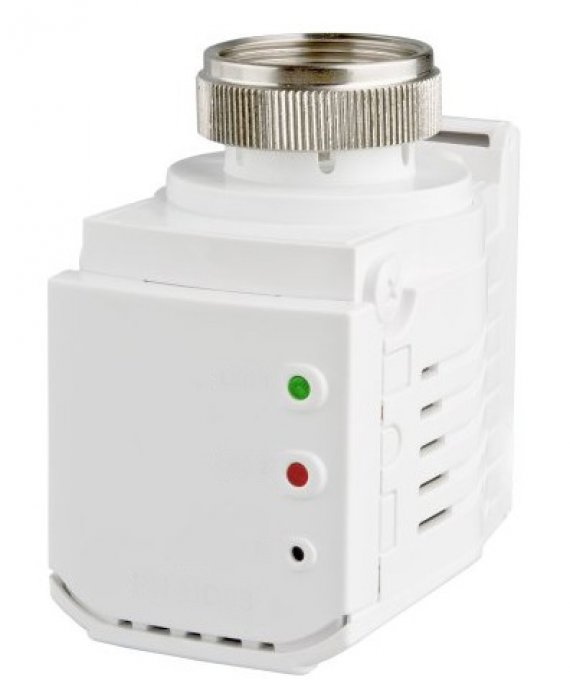
\includegraphics[scale=0.4]{obrazky-figures/m_retusovana-hlavica.jpg}
    \caption{Inteligentná hlavica MAG RA od firmy Austyn.}
    \label{fig:IQRF-TRV}
\end{figure}


Možné riešenie s~technológiou IQRF je vyskladať samostatne hlavicu ovládateľnú elektronicky a pripojiť k~nej \emph{IQRF modul}\footnote{Napríklad modul dostupný z~\url{https://eshop.iqrf.org/cz/bezdratove-moduly-tr}.}, ktorý by slúžil ako prijímač a vysielač. 
Ten by ďalej komunikoval s~\emph{IQRF bránou}\footnote{Napríklad brána dostupná z~\url{https://eshop.iqrf.org/cz/pristupove-brany}.}.  
\subsection*{LoRaWAN}
Túto technológiu využívajú dvaja výrobcovia v~dvoch konkrétnych riešeniach. Prvou je Nemecká firma \emph{Micropelt}\footnote{Stránka výrobcu \url{https://www.micropelt.com/en/}.}. 
Vyvinuli inteligentnú hlavicu\footnote{Dostupnú z~\url{https://www.smartbuildingproducts.co.uk/product/micropelt-mlr003-lorawan-actuator}.}, ktorú môžete vidieť na obrázku \ref{fig:LORA-MICROPELT}. 
Informácie o~tejto hlavici sú zo zdroja \cite{Micropelt_hlavica}. Výhodou tejto hlavice je vysoká úspora energie, nakoľko je energeticky sebestačná. 
Energiu, ktorú využíva získava konverziou teplotných rozdielov horúceho radiátora a okolitého vzduchu na elektrickú energiu. 
Tým sa eliminuje potreba častej výmeny bateríí. Hlavica ma robustný dizajn so zameraním na verejné priestory. 
Preto hlavici chýba možnosť manuálneho ovládania. Ovládanie je možné iba rádiovou LoRaWAN technológiou, ktorá je opísaná v~\ref{iot-trasport}. 
Medzi jej funkcie patrí percentuálne otvorenie ventilu alebo nastavenie konkrétnej teploty pomocou teplotného senzoru v~hlavici. 
Hlavica zároveň odosiela údaje o~teplote, stave baterky a motoru a správy o~spotrebe a generácii energie. 
V~prípade, že je spotreba dlhodobo vyššia ako generácia, je možné hlavicu cez USB port dobiť.
Najdôležitejším prvkom tohto riešenia je, že je otvorené a ponúka dokumentáciu\footnote{Dostupnú z~\url{https://micropelt.atlassian.net/wiki/spaces/MH/pages/2981889/MLR003RiEU61-07+EN}.} obsahujúcu modely a spôsoby komunikácie s~hlavicou. 
To znamená, že za použitia ľubovoľnej \emph{LoRaWAN brány} je možné po pripojení priamo ovládať hlavicu už navrhnutými príkazmi.
Inštalácia tejto hlavice ale môže obnášať komplikácie kvôli kompaktibilite s~ventilom radiátora, nakoľko pasuje iba na závit \emph{M30 x 1,5}. 
Problém môže nastať aj v~prípade častejšej komunikácie s~bránou, kedy je očakávane, že generácia energie bude nedostatočná.

\begin{figure}[H]
    \centering
    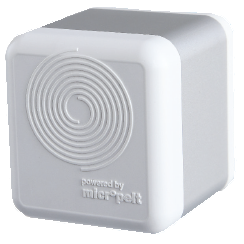
\includegraphics[scale=0.5]{obrazky-figures/_MLR003_UK-CERT_980x385_A_edited.png}
    \caption{Inteligentná hlavica MLR003 od firmy Micropelt.}
    \label{fig:LORA-MICROPELT}
\end{figure}

Druhým výrobcom je Bulharská firma \emph{MClimate}\footnote{Stránky výrobcu sú \url{https://mclimate.eu}.}. 
Táto firma vyvinula inteligentnú hlavicu\footnote{Dostupnú z~\url{https://mclimate.eu/products/vicki-lorawan}.}, komunikujúcu technológiou LoRaWAN opísanou v~\ref{iot-trasport}. Obrázok \ref{fig:LORA-MCLIMATE} zobrazuje túto hlavicu.
Informácie o~tejto hlavici sú zo zdroja \cite{vicki}.
Výhodou tejto hlavice je možnosť manuálneho ovládania, čo môže predstavovať výhodu v~prostredí domova. 
Narozdiel ale od spomínanej MLR003 od firmy Micropelt je hlavica Vicki plne závislá na batériach. 
Výrobca však sľubuje výdrž zariadenia na jeden set batérii v~období rokov. 
Medzi funkcie hlavice patrí nastavenie požadovanej teploty buď manuálne alebo diaľkovo príkazmi.
Ovládanie a reguláciu pomocou externých senzorov.
Digitálny displej zobrazujúci momentálne nastavenú teplotu. 
Možnosť zamknúť manuálne ovládanie. 
Inštalácia hlavice by nemala byť komplikovaná vďaka kompatibilite so značným počtom ventilov.
Táto hlavica je tak isto ako MLR003 je otvorená a má prístupnú rozsiahlu dokumentáciu\footnote{Dostupnú z~\url{https://docs.mclimate.eu/mclimate-lorawan-devices/devices/mclimate-vicki-lorawan}.}. 
Vďaka tomu je možné ovládanie hlavice z~rôznych aplikácii.
\begin{figure}[H]
    \centering
    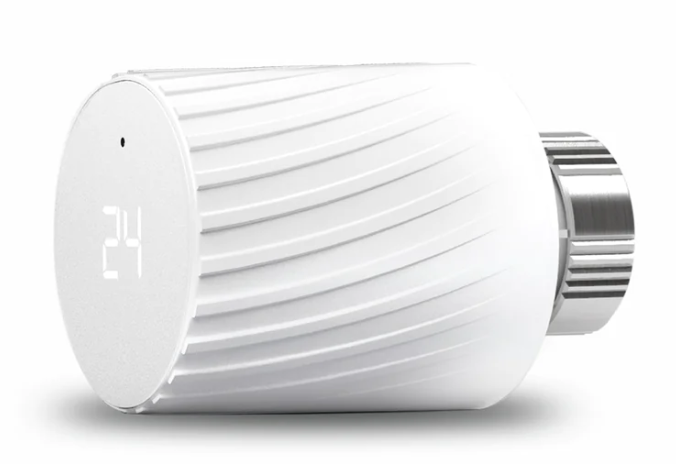
\includegraphics[scale=0.285]{obrazky-figures/vicky.png}
    \caption{Inteligentná hlavica Vicki od firmy MClimate.}
    \label{fig:LORA-MCLIMATE}
\end{figure}

\subsection*{ZigBee}
Technológia ZigBee sa pýši najväčšiemu zastúpeniu komerčných riešení. 
Táto technológia je opísaná v~kapitole \ref{iot-trasport}. 
Výrobcou riešení inteligentného vykurovania je tak isto obrovské množstvo. 
Každý ponúka trošku iné riešenie s~troška inými výhodami a nevýhodami. 
Všetky sa ale zameriavajú na prepojenie z~domácimi asistentmi alebo inými proprietárnimy aplikáciami.
Výrobcovia teda neponúkajú možnosť využiť ich riešenia a hlavice v~iných aplikáciach ako nimi podporovaných. 
Jedná sa hlavne o~\emph{Google Assistant}, \emph{Amazon Alexa}, \emph{Tuya}, \emph{Apple Siri} alebo konkrétnu mobilnú aplikáciu výrobcu na systéme \emph{Android} alebo \emph{iOS}. 
Obecne všetky takéto hlavice vyžadújú napájanie z~baterií a majú nejakú formu displeja. 
Medzi obecné funkcie patrí vzdialené ovládanie ventilu, nastavenie požadovanej teploty alebo nastavenie plánov a rozvrhov. 
Pri pripojení na domáceho asistenta získavajú radu ďalších možností, ako napríklad spustenie vyhrievania miestnosti ak sa v~nej nachádzate alebo detekcia otvorených okien a tak ďalej. 
Väčšina hlavíc nemá pri inštalácii problém, nakoľko sú väčšinou kompaktibilné so všetkými ventilmi alebo výrobcovia k~baleniu pridávajú adaptéry na ventil.
Každé riešenie od konkrétneho výrobcu výžaduje bránu od tohto istého výrobcu. 
Tým vzniká problém, kde pre ideálne riešenie je potrebné využívať produkty iba od jedného výrubcu aby nebolo potrebné mať v~domácnosti zapojených niekoľko brán. 
Tieto spomínané problémy ale ide obísť napríklad prekladom zo ZigBee komunikácie na napríklad \emph{MQTT}\footnote{Štandartný správový IoT protokol. Viac na stránkach \url{https://mqtt.org}.}, ktorému rozumie takmer každé IoT zariadenie. 
To je však proti podmienkam predajcu a k~tomu je to nabytočne komplikované.

\section{Logimic}\label{Logimic}
Jedná sa o~firmu\footnote{Dostupná na \url{https://www.logimic.com}.}, ktorá hlavne vytvára software na objednávku so zameraním na IoT aplikácie v~oblasti inteligentných miest spomínaných v~kapitole \ref{iot-smartcity}.
Klienti firmy pochádzajú z~európskych krajín a Severnej ameriky. 
Logimic pre nich vytvára rozhrania, pripravuje hardware a všeobecne inak pripravuje riešenie pre požadovaný systém. 
Jednou z~nových oblastí ktorým, by sa firma Logimic chcela venovať je aj systému pre inteligentné vykurovanie.

Na základe konverzácii s~pánom doktorom Michalom Valným a~s~pánom inžinierom Františkom Mikulu, bolo možné určiť požiadavky a očakávané výstupy firmy Logimic. 
Tá očakáva, aby v~ACADA platforme, aplikácii iTemp bolo možné ovládať a nastavovať systém vykurovania. 
Na to očakáva jednoduché a prehľadné užívateľské rozhranie. Aplikáciu iTemp môžete vidieť na obrázku \ref{fig:iTemp}.
Platforma ACADA (skratka z~anglického \emph{Asset Control and Data Acquisition}) integruje koncové zariadenia a aplikácie 3-tích strán, správu aktív, správu pracovných požiadavkou a prepojenia s~obyvateľmi mesta alebo zákazníkmi.

iTemp je bezdrôtové riešenie monitoringu vnútorného a vonkajšieho prostredia najmä teploty a vlhkosti. 
Pracuje s mnohými typmi senzorov ako je IQAROS sada, LoRa teplotné senzory a ďalšie. 
iTemp je riešenie v momentálnom neustálom vývoji a firma Logimic zadala požiadavku ho rozšíriť o ovládanie vykurovania.

\begin{figure}[H]
    \centering
    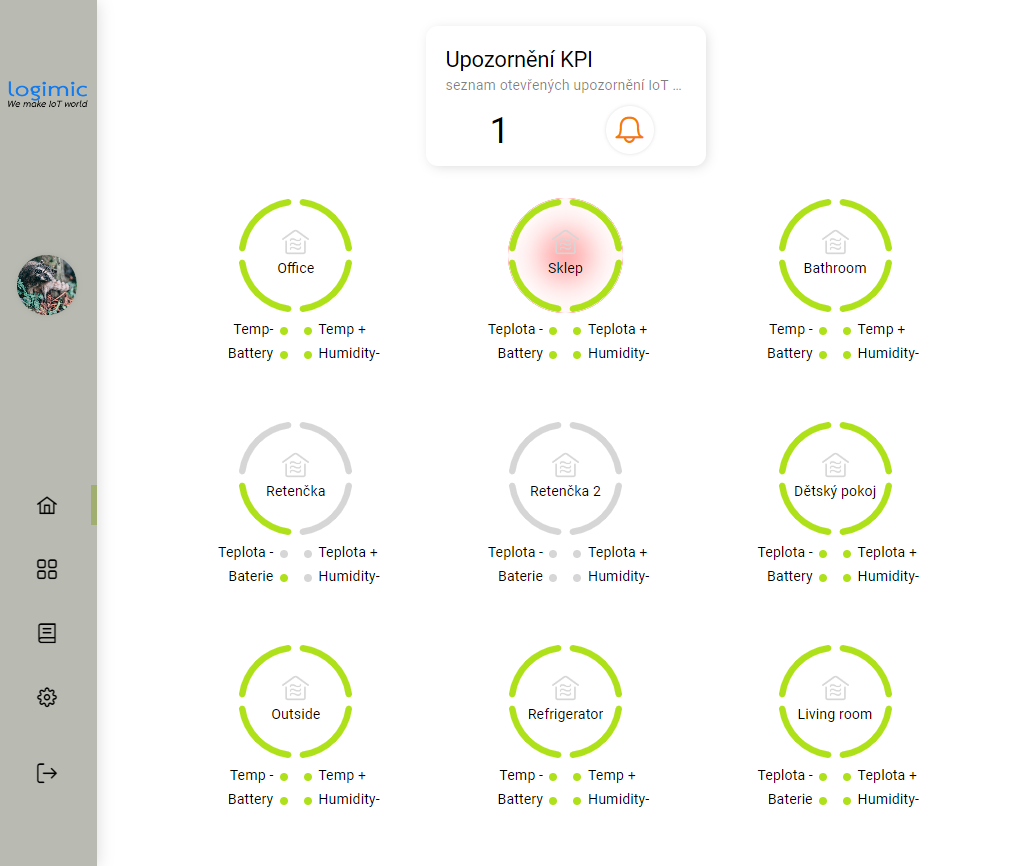
\includegraphics[width=\textwidth]{obrazky-figures/Screenshot_12.png}
    \caption{Domovská obrazovka aplikácie iTemp.}
    \label{fig:iTemp}
\end{figure}

\section{Výsledné požiadavky}\label{analyza-requirements}
Na základe analýzy potencionálnych užívateľov z~podkapitoly \ref{analyza-user} a  existujúcich riešení z~podkapitoly \ref{analyza-solutions} a konkretizovaní požiadaviek firmi Logimic z~podkapitoly \ref{Logimic} sú v~tejto kapitole vyvedené kokrétne požiadavky na systém. 
Požiadavky sú značne skresané za učelom dosiahnutia časového rozsahu bakalárskej práce.

Zameraním vývoja sa stanú byty, kde výhrevným telesom bude radiátor. 
Ten bude ovládaný regulátorom od firmy \emph{MClimate-Vicki}. 
Tým pádom bude využitá technológia \emph{LoRaWAN}. K tomu bude potreba ďalších teplotných senzorov, tiež využívajúcich technológiu LoRaWAN, aby stačila jedná brána. 
Najdôležitejšie je vytvoriť posielanie a odosielanie dát z riešenia iTemp na zariadenia. 
Pokračovať by sa malo vo vytvorení obsluhy zariadení a algoritme inteligentného vykurovania.
Funkciami inteligentného kurenia by malo byť manuálne a diaľkové ovládanie teploty v miestnosti aj za pomoci externých senzorov, možnosť zamknutia manuálneho ovládania a ovládanie teploty aj v prípade výpadku internetu.
Užívateľské rozhranie by malo vychádzať z existujúceho riešenia iTemp, rozšíreneho o odosielanie príkazov na zariadenia.
  \chapter{Návrh systémov}\label{navrh}
Celý systém vychádza a je postavený na existujúcej platforme \emph{ACADA} cloud riešenia \emph{iTemp\footnote{Dostupnej na \url{https://www.logimic.com/itemp/}.}} vytvorenej firmou \emph{Logimic}, ktorej činnosť je opísaná v~podkapitole \ref{Logimic}.
Okrem návrhu nových funkcionalít, riešení a modelov, ktoré prináša táto bakalárska práca, sú v~následujúcich kapitolách spomenuté aj už existujúce riešenia, vzory a modely riešenia \emph{iTemp}. 
V~podkapitole \ref{navrh-architektura} je vysvetlený jednoduchý koncept riešenia. 
V~nasledujúcej podkapitole~\ref{navrh-datamodel} je navrhnutý dátový model, ktorý by bol dostačujúci pre riešenie tejto bakalárskej práce.


\section{Architektúra}\label{navrh-architektura}
Na obrázku \ref{fig:designedArch}, je vidieť veľmi zjedodušený návrh zloženia architektúry. Vidno na ňom niekoľko komponentov, kde každý spĺňa určitú úlohu. Konkrétne z~prava do ľava:\begin{itemize}
    \item \textbf{\emph{Regulátor}} je \emph{IoT} zariadenie, ktoré dokáže prijímať rádiové signály a na zákade inštrukcií z~nich ovládať výkon vykurovacieho telesa.
    \item \textbf{\emph{Teplomer}} je tiež \emph{IoT} zariadenie, ktoré ale dokáže rádiovými signálmi odosielať na~ňom namerané dáta a teda v~tomto prípade najmä teplotu vzduchu v~miestnosti kde sa nachádza.
    \item \textbf{\emph{Brána}} je taktiež \emph{IoT} zariadením, ktoré fuguje ako most medzi koncovými zariadeniami a backendovým serverom. Mení internetovú komunikáciu na rádiovú a opačne.
    \item \textbf{\emph{Sieťový server}} monitoruje, spravuje a prijíma dáta od zariadení, ktoré upravuje do~lepšie spracovateľných tvarov alebo opačne do tvarov, ktorým dané \emph{IoT} zariadenia rozumejú.
    \item \textbf{\emph{Databáza}} je organizovaná kolekcie nazbieraných dát od zariadení pre vyobrazenie daných dát ale aj nastavenia regulátora a dáta pre obslúženie ďalších služieb.
    \item \textbf{\emph{Cyklická služba}} je v~podstate program, ktorý sa vykonáva nad databázov buď v~naplánovanom čase alebo ako reakcia na napríklad príchod nového nastavenia regulátora. 
    \item \textbf{\emph{Užívateľské rozhranie}} odkazuje na vizuálnu reprezentáciu nazbieraných dát od~zariadení a poskytuje grafické prostredie pre ovládanie týchto zariadení.
\end{itemize}
\begin{figure}[h!]
    \centering
    \includesvg[inkscapelatex=false,width=0.9\columnwidth]{obrazky-figures/arch_navrh.svg}
    \caption{Návrh architektúry inteligentného kúrenia.}
    \label{fig:designedArch}
\end{figure}
\section{Dátový model}\label{navrh-datamodel}
Návrh dátového modelu je na základe zjednodušeného použitia aplikácie, pri sústredení sa na riešenie inteligentnej regulácie kúrenia. Ten je možné vidieť na obrázku \ref{fig:designedModel}.
V~tomto dátovom modeli máme entitu \emph{zariadenie} s~niekoľkými atribútmi ako jeho \emph{ID}, meno, lokáciu a typ zariadenia, z~ktorého získava ďalšie parametre a príkazy. 
Každé zariadenie patrí do miestnosti, ktorú spravuje, teda meria teplotu a ovláda kúrenie. Každá miestnosť patrí pod určitý systém. 
Ten je zas vlastnený užívateľom, ktorý zariadenia, miestnosti a systémy ďalej spravuje. 
Periodicky je cyklickou službou spomenutou v~podkapitole \ref{navrh-architektura} vytvaraný pre jednotlivé zariadenia záznam s~časovou známkou. 
Tieto záznamy slúžia napríklad na vykreslovanie grafov. 
A~tak isto sú ich parametre na základe typu zariadenia, ku ktorému daný záznam patrí.
\begin{figure}[h!]
    \centering
    \includesvg[inkscapelatex=false,width=1\columnwidth]{obrazky-figures/data_model.svg}
    \caption{Návrh datového modelu inteligentného kúrenia.}
    \label{fig:designedModel}
\end{figure}
\section{Algoritmus inteligentného  kúrenia}\label{navrh-algo}
Logika algoritmu je ukrytá v~cyklickej službe, ktorá je opísaná v~podkapitole \ref{navrh-architektura}. 
Spočíva v~troch kontrolných krokoch, či sa vôbec výpočet nového stavu spustí. Podľa diagramu z~obrázka \ref{fig:ProportionalAlgLogic} ide vyčítať nasledovné tri rozhodovacie podmienky:
\begin{itemize}
    \item \textbf{Je rozdiel nameranej teploty a nastavenej teploty významný?} Znamená to, že v~prípade ak teplota kolísa v~rozmedzí 1°C podľa zdroja \cite{TemperatureSensivity}, človek nerozlíši rozdiel. 
    Pre ušetrenie zdrojov a pre dosiahnutie čo najmenšieho počtu otvárania a zatvárania ventilu je táto hranica reflektovaná aj v~logike algoritmu ale úrovňou 0,2°C. 
    V~prípade, že rozdiel nameranej a nastavenej teda cieľovej teploty je vyšší ako tepelná sensivita človeka vyhodnotí sa podmienka ako kladná a presunie sa k~ďalšej. 
    \item \textbf{Je ich rozdiel vyšší ako nastavený kritický limit?} Myslí sa tým rozdiel nameranej a nastavenej teploty. 
    V~prípade, že tento rozdiel prekročí kritický limit je potrebné zvýšiť rýchlosť vykurovania a teda otvárať ventil rýchlejšie. To sa pri kladnej odpovedi na túto otázku prejaví ako využitie vyššieho koeficientu pri výpočte otvorenia motora. Tento koeficient je opísany ďalej v~odseku o~výpočte otvorení motora.
    \item \textbf{Pohla sa nameraná teplota požadovaným smerom od poslednej kontroly?} Hlavica sa môže nachádzať v~dvoch stavoch a to kúrenia alebo chladenia. 
    Do týchto stavov sa dostáva na základe nameraných teplôt z~minulých cyklov. 
    To znamená, že ak je hlavica v~stave kúrenia a nameraná teplota z~predošlého cyklu je stále vyššia ako práve nameraná, je nutné prepočítať otvorenie motora podľa vzorca \ref{eq:MPcalculation}.
    V~opačnom prípade ak sa teplotá zdvíha znamená to, že sa blížime k~požadovanej teplote a nieje nutné prepočítavať otvorenie motora.
\end{itemize}
\begin{figure}[H]
    \centering
    %\includesvg[inkscapelatex=false,width=0.65\columnwidth]{obrazky-figures/Algo (4).svg}
    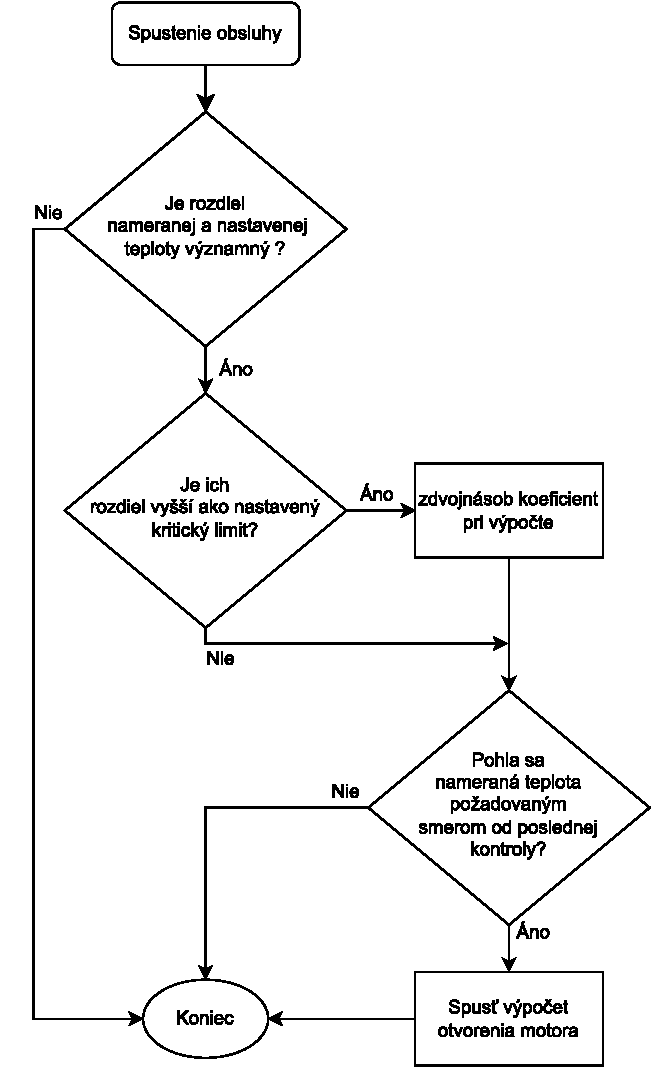
\includegraphics[width=0.65\columnwidth]{obrazky-figures/Algo (4).pdf}
    \caption{Logika inteligentného vykurovania.}
    \label{fig:ProportionalAlgLogic}
\end{figure}
\subsection*{Výpočet otvorenia motora}
Podľa následujucého vzorca \ref{eq:MPcalculation} je možné vypočítať nové otvorenia motora. 
Maximálny rozsah otvorenia motora hlavice Vicki je 0 až 800 krokov, tento rozsah sa nasledne mení podľa typu ventilu. 
Pre optimálne fungovanie hlavice je nutné zaručiť, že minimalný skok je 17 krokov inak je možné poškodenie motoru. 
Pre kalibráciu výpočtu pre miestnosti rôznych vlastností je možné použiť koeficient miestnosti v~rozsahu 0-20. 
Pre očakávané chovanie je potrebné dodržať, že cieľová teplota nesmie byť menšia ako 0.
\begin{equation}
    \centering
    \label{eq:MPcalculation}
    MP_{new} = MP_{old} - \frac{c * (T_{target} - T_{measured})*{MR}}{100}, \text{kde:}
 \end{equation}
 $MP_{new} =$ Nová pozícia motora,\\
$MP_{old} =$ Doterajšia pozícia motora,\\
$c = $ koeficient miestnosti,\\
$T_{target} = $ Cieľová teplota,\\
$T_{measured} = $ Nameraná teplota,\\
$MR = $ Maximálny rozsah motora v~krokoch,\\
\section{Komunikácia}\label{navrh-komunikacia}
Táto podkapitola sa venuje návrhu spôsobu komunikácie medzi jednotlivými komponentami z~kapitoly \ref{navrh-architektura} obrázka \ref{fig:designedArch}. Na najnižšej části, teda v~části komunikácie medzi \emph{IoT} zariadeniami, navrhujem využiť služby bezdrátového \emph{LoRaWAN} protokolu. 
Tieto zariadenia, konkrétne teda spomínaný \emph{regulátor}, \emph{teplomer} a \emph{brána} si medzi sebou budú vymieňať \emph{LoRaWAN dátové rámce}. Brána LoRa rádiové signály dešifruje a prepošle na LoRaWAN sieťový server štadartným sieťovým protokolom \emph{UDP} alebo \emph{MQTT\footnote{Viac informácii o~tomto protokole na \url{https://mqtt.org}.}}. 
Server užitočné dáta od zariadení prijíma zašifrované v~kódovaní \emph{BASE64}. 
To musí dekódovať, v~tomto prípade do hexadecimálneho kódovania. K~nemu na základe dokumentácie \emph{regulátoru} a \emph{teplomeru} je potrebné vytvoriť dekóder pre prichádzajúce správy od zariadení a kóder pre správy smerujúce na zariadenia. 
Výstupom dekódera a teda aj vstupom kódera je správa vo formáte \emph{JSON\footnote{Viac informácii o~tomto formáte na \url{https://www.json.org/json-en.html}.}.}
Táto správa je cez \emph{MQTT} poslaná ďalej na databázu, kde je správa spracovaná a uložená do databázy. 
Nad databázov bude bežať \emph{cyklická služba} s~priamým prístupom do databázy. Užívateľská aplikácia pristupuje k~databáze cez \emph{REST-API}.

\section{Užívateľské rozhranie}
Riešenie užívateľského prostredia je poskytnuté existujúcim riešením \emph{iTemp}.
Riešenie spočíva v~trojvrstvom modeli, kde s~vyššou vrstvou zachádzame do vyšších detailov. Vrstvy sú následovné:
\begin{itemize}
    \item \textbf{Layer 1} (L1), alebo prvá vrstva. Táto vrstva uchováva nastavené skupiny, kde vyobrazuje \textit{kľúčové ukazatele výkonnosti} (KPI) \cite{eckerson2010performance}. Pre užívateľskú prívetivosť sú reprezentované ako farebné štvrť kružnice okolo obrázka reprezentujúceho danú skupinu, v~tomto prípade miestnosť. Farbou sa označuje situácia v~akej sa skupina nachádza. Dané situácie sa dajú nastaviť podmienkami v~nastaveniach KPI.
    \item \textbf{Layer 2} (L2), alebo druhá vrstva ponúka bližší detail na danú skupinu s~vyšším detailom na KPI, dôležité parametry skupiny, príkazy volané nad skupinou a konkrétne zariadenia priradené do tejto skupiny.
    \item \textbf{Layer 3} (L3), alebo tretia vrstva. V~poslednej vrstve máme konkrétne zariadenia, ktoré majú detail s~väčšinou dôležitých informácii, majú svoj profil obsahujúci ich aktuálne parametre, aktívne upozornenia z~KPI, dokumentáciu o~zariadení, poslednú správu ktoré zariadenie poslalo na server, konkrétne parametre s~možnosťou editácie a nakoniec štatistiku parametrov zobrazenú v~grafoch.
\end{itemize}
  \chapter{Implementácia}\label{impl}
Implementácia začala komunikáciou s~firmou \emph{Logimic} opísanou v~kapitole \ref{Logimic}. Tá mi poskytla senzory \emph{RisingHF1S001} s~proprietárnou \emph{TTI bránou} firmy \emph{The Things Industries\footnote{Viac o~firme na stránkach \url{https://www.thethingsindustries.com}.}}. 
Obe zariadenia sú pre LoRaWAN riešenia. 
Implementácia sa teda ďalej, ako podľa plánu, sústredí na túto technológiu. 
Nanešťastie v~priebehu implementácie sa firma \emph{Logimic} rozhodla ukončiť spoluprácu s~\emph{The Things Industries} a musel som svoju prácu migrovať inam a teda začínať nanovo. 
Táto kapitola ďalej pokračuje od tohto momentu a prechádza implementáciou na základe hlavných komponentov architektúry z~kapitoly \ref{navrh-architektura}. 
Teda podkapitola \ref{impl-IOT} sa venuje všetkým využitým \emph{IoT} zariadeniam, ich inštalácii a konfigurácii. 
Podkapitola \ref{impl-Chirp} sa venuje LoRaWAN sieťovému serveru (ďalej využívana skratka LNS), na ktorom sú zariadenia zaregistrované. Ďalej sa venuje kóderu a dekóderu, ktoré na ňom pracujú. 
Následne, podkapitola \ref{impl-Lambda} sa venuje cyklickej službe. Nakoniec podkapitola \ref{impl-iTemp} vysvetľuje postup prípravy užívateľskej aplikácie \emph{iTemp} na toto riešenie.

Celá implementácia je vytvorená v~integrácii s~riešením \emph{iTemp}. To znamená, že nie je presne podľa návrhov z~kapitoli \ref{navrh}. 
Napriek tomu je návrh stále podobný implementácii. Všetky konfiguračné súbory, kódy a programy vytvorené pre túto bakalársku prácu sú dostupné na \emph{GitHub}\footnote{Konkrétny link je \url{https://github.com/Siki-ux/bp-int-heating}.}.


\section{IoT zariadenia}\label{impl-IOT}
Následujúce podkapitoly sa venujú konkrétnym zariadeniam použitých pri implementácii. Všetky zariadenia boli poskytnuté firmou \emph{Logimic}.
\subsection{RisingHF1S001}\label{impl-Rising}
Je to \emph{LoRaWAN} bezdrátový senzor teploty a vlhkosti vyrábaný firmou \emph{RisingHF\footnote{Viac o~firme na stránkach \url{https://www.risinghf.com/home}.}}. 
Toto kompaktné zariadenie pracujúce na batériach môže byť inštalované v~rôznych podmienkach na rôznych miestach. 
V~tomto prípade bude slúžiť hlavne ako teplotný senzor umiestnený v~miestnosti na mieste, kde chce užívateľ dosiahnuť požadovanú teplotu.
\subsection*{Inštalácia}
Inštalácia tohto zariadenia je jednoduchá a spočíva iba v~uvoľnení šrúb vonkajšieho obalu a zapojení batérie.
\subsection*{Konfigurácia}
Konfigurácia vyžaduje proprietárny konfiguračný nástroj \emph{RCFG Tool} firmy \emph{RisingHF}. Zariadenie zbavené vonkajšieho obalu pripojíme USB-mini B káblom k~počítaču. Následne spustíme konfiguračný nástroj. Ním môžme nahrať do zariadenia konfiguračný súbor. Mimo iné je v~ňom najdôležitejšie nakonfigurovať komunikačné kanály, kľúč aplikácie (\emph{AppKey}) pre aktiváciu vzduchom (\emph{OTAA}) a zabezpečenie komunikácie. 

\subsection{MClimate Vicki LoRaWAN}\label{impl-Vicki}
Toto zariadenie je bližšie opísané v~kapitole \ref{analyza-solutions} v~části o~technológii \emph{LoRaWAN}. Pri začiatku implementácie vyšlo toto zariadenie ako najvýhodnejšie.
\subsection*{Inštalácia}
Najskôr je potrebné odpojiť zadný kryt hlavice. 
Ten následne pripojiť na termostatický ventil. Do samotnej hlavice následne zapojiť batérie. Počkať na svetelnú signalizáciu hlavice a~následne ju pripojiť k~zadnému  krytu na termostatickom ventile. Zariadenie následne prejde do kalibračného režimu na niekoľko minút. Po zobrazení nastavenej teploty na displeji je kalibrácia hotová a zariadenie je pripravené na prácu.
\subsection*{Konfigurácia}
Zariadenie prichádza predkonfigurované s~konfiguráciou zameranou na aplikáciu \emph{MClimate Enterprise\footnote{Viac informácii na \url{https://mclimate.eu/pages/enterprise}.}}. Z~tejto aplikácie je možné prenastaviť predvolený \emph{LoRaWAN} server na server \emph{Chirpstack}, ktorý je opísaný v~nasledujúcej podkapitole \ref{impl-Chirp}.


\subsection{Mikrotik wAP LR8}
Jedná sa o~bedrátový prístupový bod (\emph{AP}) produkovaný firmov \emph{Mikrotik\footnote{Viac informácii o~firme na \url{https://mikrotik.com}.}}. Má množstvo funkcii\footnote{Zoznam dostupný na \url{https://mikrotik.com/product/wap_lr8_kit}.}, no pre riešenie tejto práce sú relevantné najmä: možnosť prijímať LoRaWAN komunikáciu a možnosť použiť ho ako most medzi \emph{Chirpstack} serverom, opísanom v~podkapitole \ref{impl-Chirp} a \emph{IoT zariadeniami}, opísaných v~podkapitole \ref{impl-IOT}.
\subsection*{Inštalácia}
Spodný kryt zariadenia je zabezpečený jednou skrutkou. 
Po jej odšrubovaní sa ukáže priestor na pripojenie zdroja energie, ethernetový port a port antény. 
Následne sa pripojí anténa a ako zdroj energie použijeme technológiu \emph{PoE} (Power over ethernet), teda zdroj energie pôjde pripojeným ethernetovým káblom. Následne zasunieme zadný kryt a~zaistíme ho skrutkou.
\subsection*{Konfigurácia}
Zariadenie funguje ako prístupový bod. Vďaka tomu sa na neho dá pripojiť technológiou \emph{Wi-fi} a prístupom na adresu \emph{192.168.88.1}. 
Tak sa dá dostať do ovládacieho rozhrania zariadenia. V~sekcii \emph{LoRa} vytvoríme pripojenie na LNS a zapneme službu tejto brány. 
V~tomto momente začne zariadenie prijímať LoRa správy a bude ich ďalej posúvať na LNS.  


\section{Registrácia zariadení}\label{impl-Chirp}
 Zariadenia je potrebné registrovať na LoRaWAN sieťový server.
 K tomu bol zvolený Chirpstack.
 Ten je open-source LoRaWAN sieťový server a aplikačný server, ktorý poskytuje kompletné riešenie na budovanie, nasadzovanie a spravovanie LoRaWAN sietí. 
 S~jeho využitím je možné jednoducho vytvárať vlastné aplikácie pre monitorovanie, riadenie a správu LoRaWAN zariadení a senzorových dát.
 ChirpStack umožňuje aj vytvorenie rozšíriteľných IoT riešení a ich integráciu do existujúcich systémov a cloudových platform, teda riešenia firmy \emph{Logimic}. 
 Podstatnou časťou platformy Chirpstack je preklad surových neformátovaných dát na dáta zrozumiteľné pre cloudové riešenie \emph{iTemp}. 
 K~tomu sa využívajú dva programy spoločne označované ako \emph{Codec}, patriace konkrétnym typom zariadení. Sú to kóder a dekóder, ktoré sú opísané ďalej.
\subsection*{Kóder}
Jedná sa o~program, ktorý sa spustí nad príchodzími datami z~aplikácie a vytvára preklad do formy pochopiteľnej pre zariadenie, ktoré týmto príkazom bude ovládať. V~tomto riešení sú vstupné dáta vo formáte JSON a výstupom je správa vo formáte \emph{Base64}. Chirpstack preklad do \emph{Base64} vytvára sám a požaduje k~tomu aby výstup kódera bol reťazec v~číselach desiatkovej sústavy o~veľkosti jedného bajtu.

To sa dá dosiahnúť postupným rozoberaním vstupnej JSON správy. Kde sa  podľa návrhu očakáva, že pod kľúčom \texttt{cmdName} sa nachádza názov príkazu, ktorý sa má vykonať. 
Prepínačom sa rozdelí do konkrétnej obsluhy daného príkazu, kde ďalej očakáva že pod kľučom \texttt{cmdPars} budú jednotlivé parametry daného príkazu. Následne sa do reťazca postupne pridá kód daného príkazu a vyformátované parametre. Prípadne je vykonaná kontrola vstupných parametrov, kde je možné, že by nesprávna hodnota mohla poškodiť zariadenie.

\subsection*{Dekóder}
Jedná sa o~program, ktorý sa spustí nad prichádzajúcimi datami od zariadení a vytvára preklad do formy pochopiteľnej pre aplikáciu a databázu. Dekóder dostáva vstupné dáta ako čísla v~desiatkovej sústave o~veľkosti jedného bajtu v~reťazci. Výstupom je zas správa vo formáte JSON v~štruktúre vytvorenej a vyžadovanej aplikáciou opísanou v~podkapitole \ref{impl-iTemp}.

To sa dá dosiahnuť dešifrovaním prvého čísla reťazca na jednotlivé parametre na základe implementácie zariadenia výrobcom. Ďalej podľa parametru nasledujúci určitý počet čísel v~reťazci patrí danému parametru a reprezentuje jeho hodnotu. Ak sa ďalej nachádzajú ďalšie čísla znamená to, že následuje ďalší parameter a proces sa opakuje. Tieto parametre sa postupne zapisujú pod kľúč \texttt{devPars} pod ich vlastým kľúčom.

\section{Obsluha zariadení}\label{impl-Lambda}
Jedná sa o~cyklickú službu \emph{AWS Lambda\footnote{Viac informácii o~službe na \url{https://aws.amazon.com/lambda/}.}}, ktorá spúšťa určité funkcie ako reakciu na napríklad prichádzajúce data alebo ich spúšťa v~určitom časovom intervale. V~tomto riešení je funkcia \texttt{HeatingControl} volaná v~intervale 5 minút. To z~dôvodu potreby zariadenia spraviť dva cykly správ \emph{keep-alive}. \emph{Keep-alive} je správa, ktorú hlavica posiela periodicky v~intervale 2 minút. Správa obsahuje potrebné informácie na výpočty funkcie \texttt{HeatingControl}. Dôvod potreby dvoch cyklov spočíva v~tom, že prvá správa potvrdí príjem zaslaného príkazu a druhá zašle aktuálne dáta na databázu.

Funkcia \texttt{HeatingControl} sa pred zavolaním pripojí do databázy \texttt{iTemp2}, čo je ostrá databáza riešenia \emph{iTemp}. 
Po úspešnom naviazaní spojenia si funkcia získa všetky hlavice, ktoré má ovládať.
Ako ukazuje diagram na obrázku \ref{fig:diagram}, dosiahne to prístupom do databázy funkciou \texttt{getDeviceList} s identifikačným číslom (ďalej používaná skratka ID) modelu hlavice, ktorá následne vráti list hlavíc.  
Z neho je pre každú hlavicu získané konkrétne ID systému, v ktorom sa hlavica nachádza a ID konkrétnej hlavice.
Každá hlavica sa nachádza v nejakej skupine, ktorá reprezentuje miestnosť, v ktorej je nainštalovaná. Preto je potrebné získať skupiny, v ktorých sa nachádza ďalším prístupom do databázy. 
To funkciou \texttt{getGroupList} s parametrom ID systému a ID hlavice, ktorá vráti list skupín tohto systému, v ktorých je hlavica nainštalovaná. Následne je možné pre každú ovládanú miestnosť získať z databázy konkrétne hodnoty parametrov ovládanej miestnosti. 
To funkciou \texttt{getDeviceParameterValueList} s parametrom ID hlavice, ktorá vráti list obsahujúci všetky parametry danej hlavice. 
Skupina, teda miestnosť môže používať externé teplotné senzory. K tomu je použitá funkcia \texttt{getRoomTemp}, ktorá v prípade že nájde v miestnosti teplotné senzory, vypočíta z ich nameraných teplôt priemer. 
Ak miestnosť nepoužíva teplotné senzory vráti hodnotu nameranú na hlavici.

Na základe získaných parametrov funkcia \texttt{HeatingControlLogic} začne vyhodnocovať situáciu. To spôsobom opísaným v podkapitole \ref{navrh-algo}. Teda najprv skontroluje, či je vôbec nutné spúšťať výpočet na základe rozdielu nameranej a cieľovej teploty. 
Ak je rozdiel dostatočný zistí, či je potrebné miestnosť vyhriať alebo  
naopak ochladiť. 
Ďalej sa skontroluje, či sa teplota od minulého cyklu pohla požadovaným smerom. Ak áno, nieje potrebné upraviť pozíciu motora. Ak nie, je potrebné prepočítať otvorenie motora na hlavici. 
Tento výpočet zabezpečuje funkcia \texttt{HeatingAlgo} volaná s parametrami miestnosti. 
Tá vypočítava pozíciu motora na základe vzorca \ref{eq:MPcalculation}. 
K tomu kontroluje, či je výsledok výpočtu a pôvodné nastavenie rozdielne o minimálny rozdiel krokov motora určeného v podkapitole \ref{navrh-algo}. 
Ak nie je, funkcia vráti pôvodné nastavenie. 
V prípade, že je výsledok mimo hranice motora, funkcia vráti najbližšiu hranicu. 
Funkcia \texttt{HeatingControlLogic} po získaní pozície motora vráti list s potrebnými datami. 
Z tohto listu sa ešte raz získa pozícia motora, ktorá sa porovná s predošlou pozíciou motora. 
V prípade, že nie sú rovnaké vyšle sa príkaz funkciou databázy \texttt{putLaunchCmdDevice} s parametrami ID hlavice, ID požadovaného príkazu a listom získaným z funkcie \texttt{HeatingControlLogic}. Následne je už len potrebné aktualizovať data v databáze. To funkciou \texttt{updateLastValue}, ktorá pripraví data do databázy a funkciou databázy \texttt{putDeviceParameterValueList} aktualizuje naposledy nameranú teplotu na momentálne nameranú teplotu.

 Funkcia \texttt{HeatingContorlLogic} je volaná nad každou hlavicou.
 Funkcia \texttt{HeatingControl} nakoniec vráti status 0, znamenajúci úspešné ukončenie ovládania.

\begin{figure}[H]
    \centering
    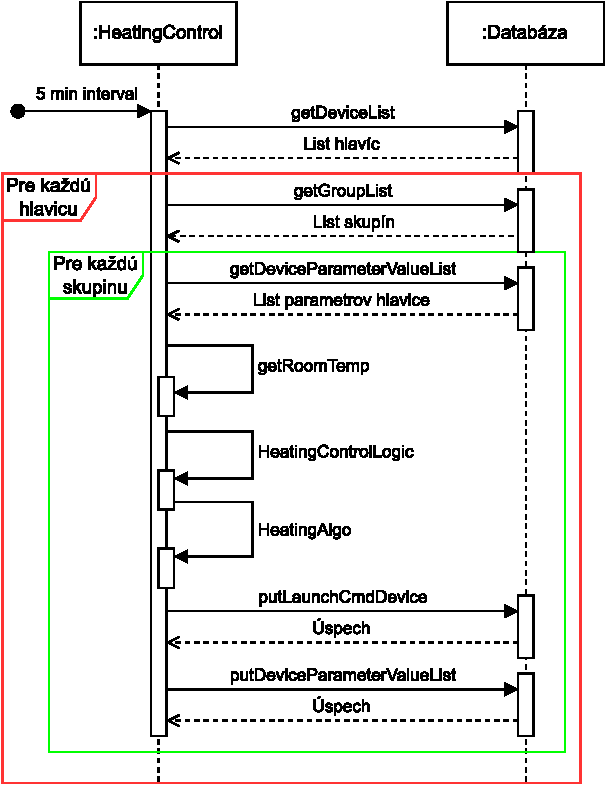
\includegraphics[width=0.8\textwidth]{obrazky-figures/diagram.pdf}
    \caption{Diagram služby ovládania kúrenia.}
    \label{fig:diagram}
\end{figure}

\section{Užívateľská aplikácia}\label{impl-iTemp}
Tou sa stala aplikácia iTemp.
Tá predstavuje bezdrôtové riešenie monitoringu vnútorného a vonkajšieho prostredia najmä teploty a vlhkosti.
Pracuje s~mnohými typmi senzorov ako je IQAROS sada\footnote{Viac informácii na \url{https://iqaros.cz/custom.html}}, LoRa teplotné senzory a ďalšie. 
Informácie máte v~telefóne, tablete, alebo domácom touch screene. Systém nielen monitoruje ale tiež informuje o~prekročených hodnotách a ukladá dlhodobo štatistiky.

V~rámci tohto riešenia je potrebné využitie \emph{SQL nástroja}  v~module administrácie. 
Tu sa vytvárajú typy parametrov, parametre a ich napríklad jednotky, ktoré sa skladajú do do modelov zariadení. Model zariadenia Vicki je možné vidieť na obrázku \ref{fig:model}.
Takýmto spôsobom sa pripraví databáza pre zariadenie a zadefinujú konktrétne kľúče \emph{JSON} správ. 
Následne je potrebné vytvoriť modely príkazov, ktoré budú posielané na zariadenie. 
Skladajú sa z~parametrov, ktoré budú upravovať a vytváraju tak \emph{JSON} správu, ktorej \emph{kóder} z~podkapitoli \ref{impl-Chirp} rozumie a po preložení ju zašle na zariadenie. 
Príkazy je potrebné ďalej priradiť konkrétnym zariadeniam.

Po príprave databázy, následuje založenie skupín, teda pre toto riešenie miestností, ktoré chceme ovládať zariadeniami. 
To sa vykonáva tak isto v~administrátorskom module. 
V~tomto konkrétnom riešení je ovládaná jedna miestnosť s~jedným regulátorom a dvoma tepelnými senzormi. 
Voliteľne je možné si nastaviť \emph{KPI} skupiny pre lepší prehľad z~domovskej obrazovky. V~tomto momente je regulácia teploty v~miestnosti ovládaná obsluhov z~predchádzajucej  kapitoly \ref{impl-Lambda}.

Pre zobrazenie konkrétnych dát, štatistík, grafov a zaslaných príkazov je potrebné prejsť cez skupinu na konkrétne zariadenie.

\begin{figure}[H]
    \centering
    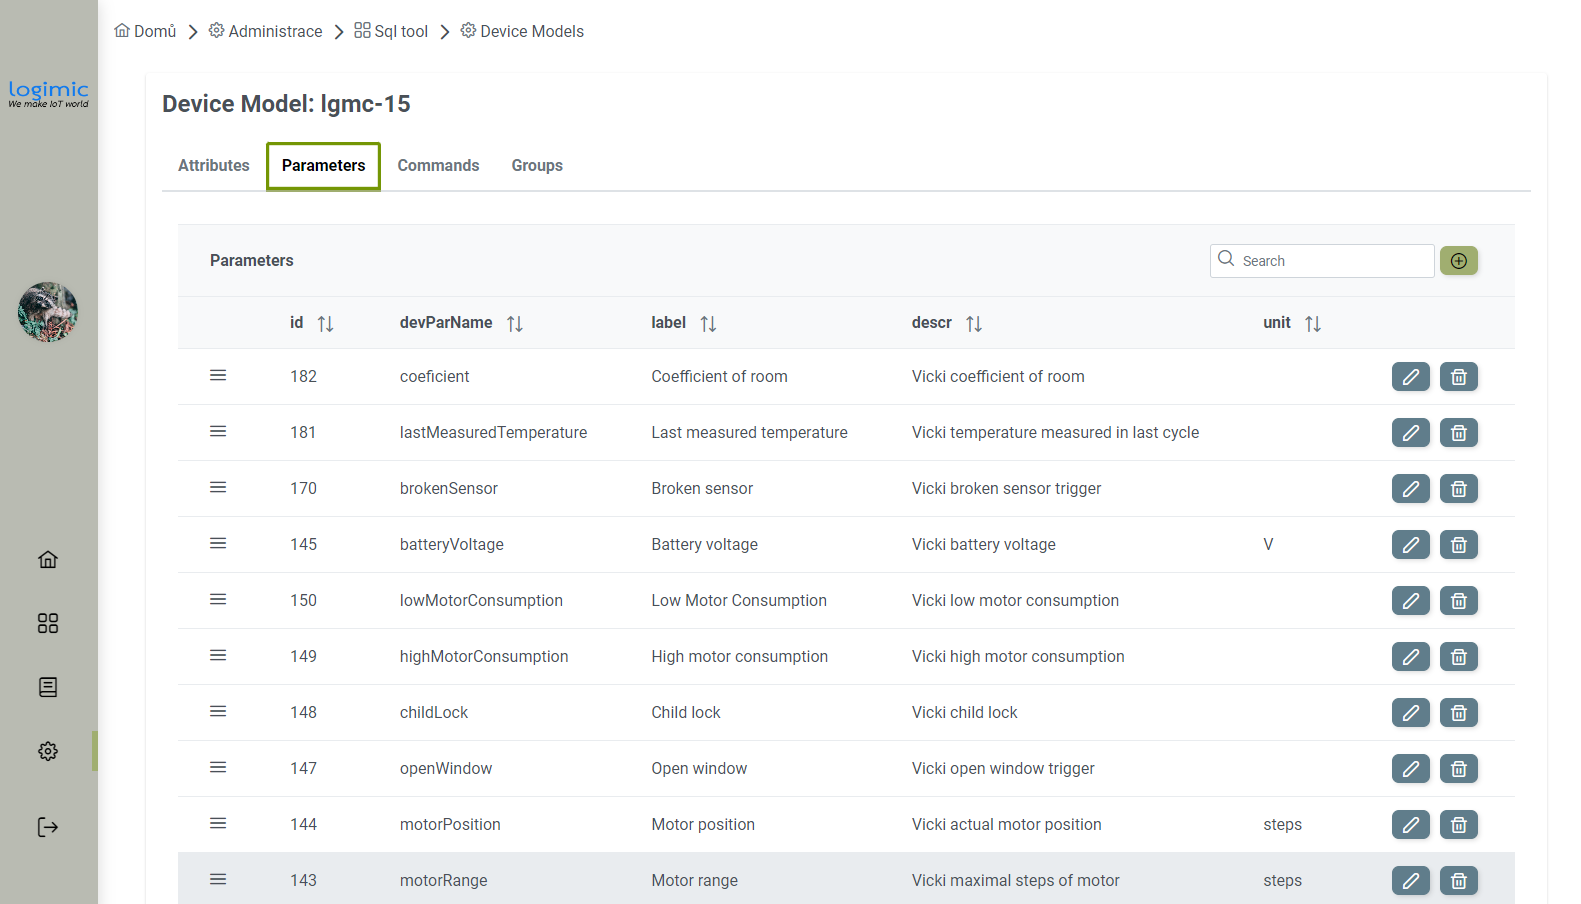
\includegraphics[width=\columnwidth]{obrazky-figures/Screenshot_13.png}
    \caption{Model zariadenia Vicki v SQL nástroji aplikácie iTemp.}
    \label{fig:model}
\end{figure}
  \chapter{Testovanie}\label{test}
Testovanie prebiehalo v~dvoch prostrediach. 
Jedným bolo simulované prostredie, ktorého zameraním bolo overiť funkciu algoritmu a logiky ovládania inteligentného vykurovania. Opísané v~podkapitole \ref{test-sim}.
Druhým prostredím bolo reálne prostredie, teda konkrétna miestnosť ovládaná inteligentným vykurovaním. 
Proces tohto testovania, jeho detaily a~výsledky sú opísané v~podkapitole \ref{test-real}.

\section{Testovanie v~simulovanom prostredí}\label{test-sim}
Toto prostredie bolo vytvorené nad implementovaným algoritmom. 
Implementáciu simulácie je možné nájsť na stránkach \emph{GitHub\footnote{Konkrétny odkaz je \url{https://github.com/Siki-ux/bp-int-heating/tree/main/test_algo}.}.}
Ten bol napojený na fiktívnu databázu reprezentovanú statickými údajmi. 
Hlavnou časťou simulácie bol cyklus reprezentujúci cyklickú obsluhu s~intervalom 5 minút. 
Vývoj teploty prostredia bol simulovaný pseudonáhodnými číslami, ktoré predstavovali pohyb teploty.
To znamená, že teplota v~miestnosti klesá o~náhodnú teplotu, z~limitu každý cyklus, pričom vzácne môže teplota aj stúpnuť.
Tento pohyb bol ďalej modifikovaný do tvaru goniometrické sínusoidy s~periódou 24 posunutou o~8 hodín.
To s~cieľom simulovať priebeh teploty počas dňa.
V~simulácii bolo možné nastaviť všetky podstatné premenné inteligentného vykurovania, počiatočné body simulácie a koeficienty vyhrievania, chladenia a goniometrickej funkcie.
Dva simulované senzory \emph{RisingHF1S001}, opísané v~podkapitole \ref{impl-Rising}, odosielali teplotu do simulovanej databázy každý cyklus.
Po~zavedení simulovaného regulátoru \emph{Vicki}, opísaného v~podkapitole \ref{impl-Vicki}, je stúpavý pohyb teploty navýšený o~výkon výhrevného telesa.
Regulácia, teda pohyb motora, čo má za následok zvýšenie alebo zníženie výkonu výhrevného telesa, je vypočítavaná v~rovnakom cykle.
Výstupom simulácie je tabuľka meraných veličín, ktorá bola väčšinou vizualizovaná na grafe v~programe \emph{MS Excel}.

Počas testovania bolo otestovaných niekoľko systémov ovládania regulácie vykurovania. 
Patril medzi nich aj robustný \emph{PID systém}, ktorý však nebolo možné efektívne implementovať do riešenia \emph{iTemp} a zároveň jeho výsledky, aj napriek rozsiahlemu testovaniu s~rôznymi vstupmi, nepreukázali požadované výsledky.
Zapríčinené to mohlo byť aj nie najlepším návrhom simulovaného prostredia.
Najideálnejšie výsledky v~širšom časovom pásme preukázal pôvodne navrhovaný algoritmus opísaný v~podkapitole \ref{navrh-algo}.

Na obrázku \ref{fig:simGraph}, je možné vidieť výstup jedného z~testov. 
Tento test začínal na počiatočnej teplote 20°C v~48 hodinách. 
Násobok úbytku teploty bol 1 a vyhrievania bol 8. 
Algoritmus používal koeficient 5. 
Na základe grafu je možné vidieť, že algoritmus splnil požiadavky aby maximálny rozdiel nameranej a požadovanej teploty bol 1°C a použil k~tomu malý počet pohybov motora. 
Algoritmus čiastočne sínusoidu vyrovnal, čo sa dá porovnať s~obrázkom \ref{fig:simGraphNoHeating}, kde je vyobrazený priebeh bez spusteného vykurovania.

\begin{figure}[H]
    \centering
    \includesvg[inkscapelatex=false,width=0.9\textwidth]{obrazky-figures/simGraph.svg}
    \caption{Graf teplôt a pozície motora v~simulácii.}
    \label{fig:simGraph}
\end{figure}

\begin{figure}[H]
    \centering
    \includesvg[inkscapelatex=false,width=0.9\textwidth]{obrazky-figures/simGraphNoHeating.svg}
    \caption{Graf vývoja teploty v~simulácii.}
    \label{fig:simGraphNoHeating}
\end{figure}



\section{Testovanie v~reálnom prostredí}\label{test-real}
Toto testovanie prebiehalo v~jednej miestnosti bytu vo vežiaku. 
Testovacie prostredie, teda miestnosť bola o~rozlohe $12.2 m^2$ s~jedným výhrevným telesom. 
Tým bol liatinový radiátor, napojený na ústredný zdroj tepla. 
Na ventil radiátora bola napojená inteligentná hlavica \emph{Vicki} opísaná v~podkapitole \ref{impl-Vicki}. 
Nad radiátorom sa nachádzalo plastové dvojokno. 
Dvere miestnosti boli situované do uzavretého priestoru a nachádzali sa oproti oknu s~radiátorom. 
Pre účely testovania boli použité dva tepelné senzory \emph{RisingHF1S001} opísané v~podkapitole~\ref{impl-Rising}. 
Prvý bol umiestnený v~blízkosti okna a radiátora a druhý bol umiestnený približne v~strede miestnosti vo výške $1.2 m$.
Všetky tri zariadenia spadali pod rovnaký systém a boli umiestnené do rovnakej skupiny, teda miestnosti.
Koeficient miestnosti bol nastavený na 3.
Zariadenia monitorujúce a ovládajúce teplotu v~miestnosti sú odfotené na~obrázkoch \ref{fig:test_device}.

Po spustení zariadení a nastavení požadovanej teploty aplikáciou \emph{iTemp} podľa obrázka~\ref{fig:test_setTarget}, začala rutina ovládať túto miestnosť. 
To sa postupne prejavilo na štatistikách zariadení v~miestnosti. 
Konkrétne bolo najdôležitejšie zariadenie \emph{Vicki}, teda hlavica ovládajúca ventil. 
Grafy vývoja teplôt a otvorenia ventilu z~noci 28. apríla na~29. apríl sú zobrazené na~obrázkoch~\ref{fig:test_itempStat}. 
Na prvý pohľad vyzerá ovládanie v~poriadku, podľa očakávaní. 
Po exporte dát do \emph{Excelu} a ich podrobnejšom skúmaní a priblížení je možné ale odhaliť chybu. 
Tú môžete vidieť na~obrázku \ref{fig:statisticGraph}.
Z~neho je možné vyčítať časté kmitavé pohyby pozície motora.
Vďaka tomuto problému bolo možné na základe bližšieho skúmania tejto anomálie odhaliť zaokrúhľovaciu chybu v~algoritme. 
Teplotné senzory pracovali na vysokej presnosti a tak aj extrémne malé rozdiely zapríčinili uzavretie alebo otvorenie ventilu. 
Po~oprave tejto a niekoľkých ďalších menších chýb, ktoré neodhalila simulácia, je na obrázku~\ref{fig:statisticGraph01} vidieť ďalší graf. 
Ten je z~dňa 4. mája v~časovom intervale od 2:00 do 9:00. 
Na ňom vidno takmer perfektný priebeh vývoja teploty a pozície motora.
V~momente poklesu teploty sa spustilo vyhrievanie, ktoré nepresiahlo limity požadovanej teploty, využilo minimálny počet pohybov motora a zároveň aj našlo rovnovážny bod medzi otvorením motora a teploty.

\begin{figure}[H]
    \centering
    \begin{subfigure}[b]{0.45\textwidth}
        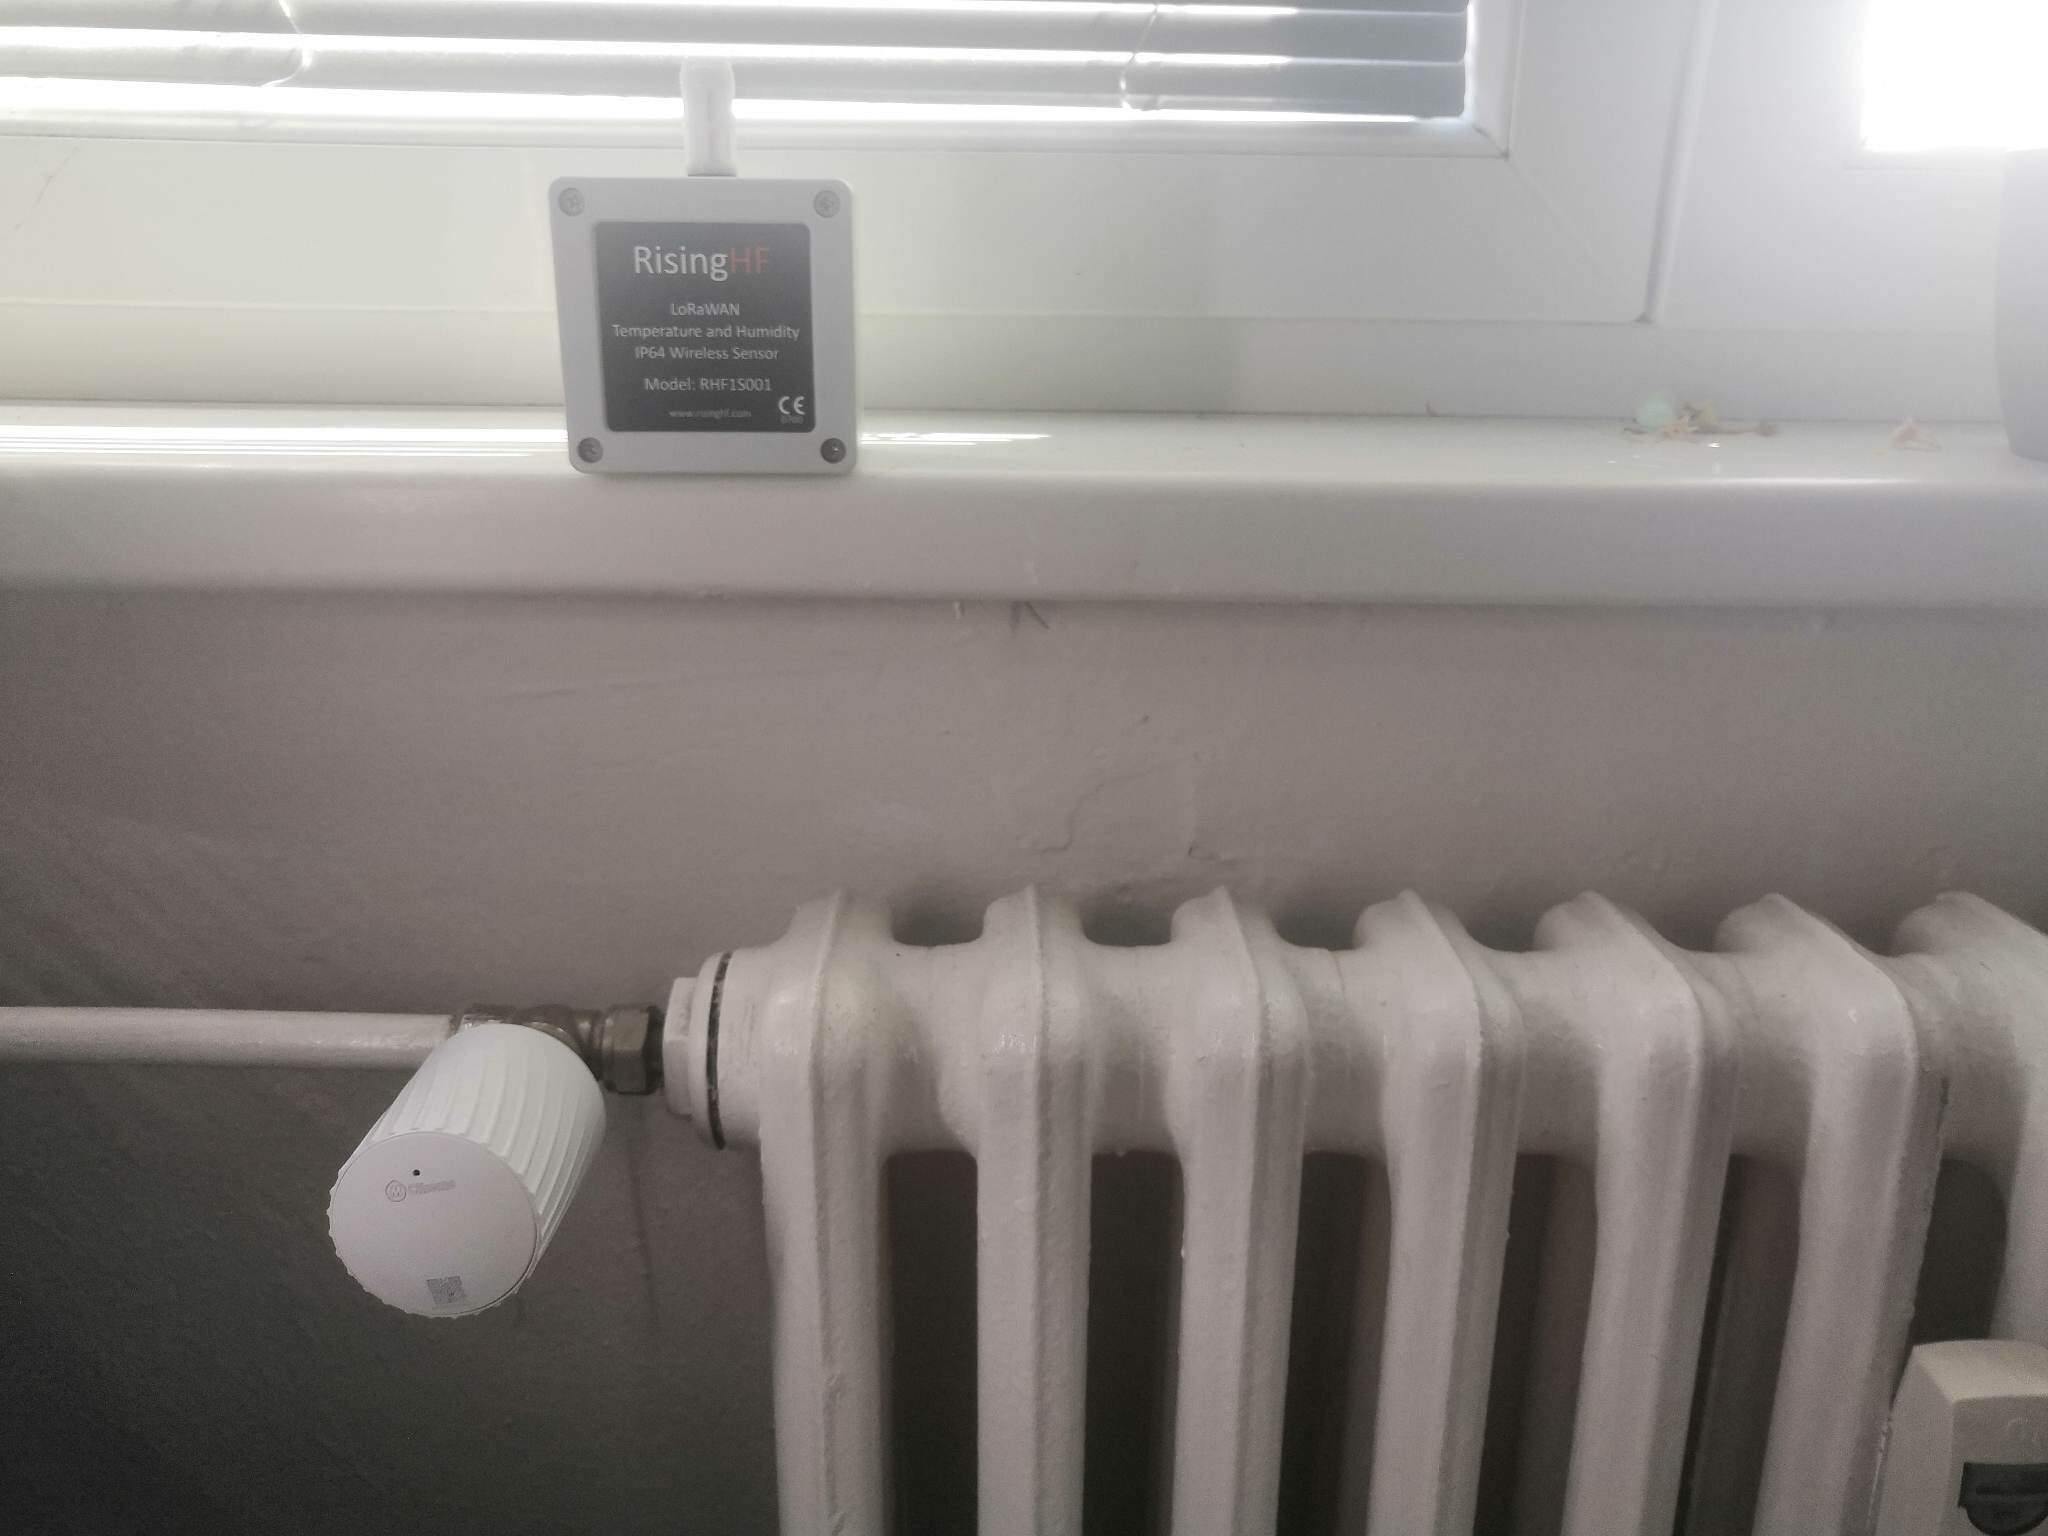
\includegraphics[width=\textwidth]{obrazky-figures/dev_picture_1.jpg}
    \end{subfigure}
    \begin{subfigure}[b]{0.45\textwidth}
        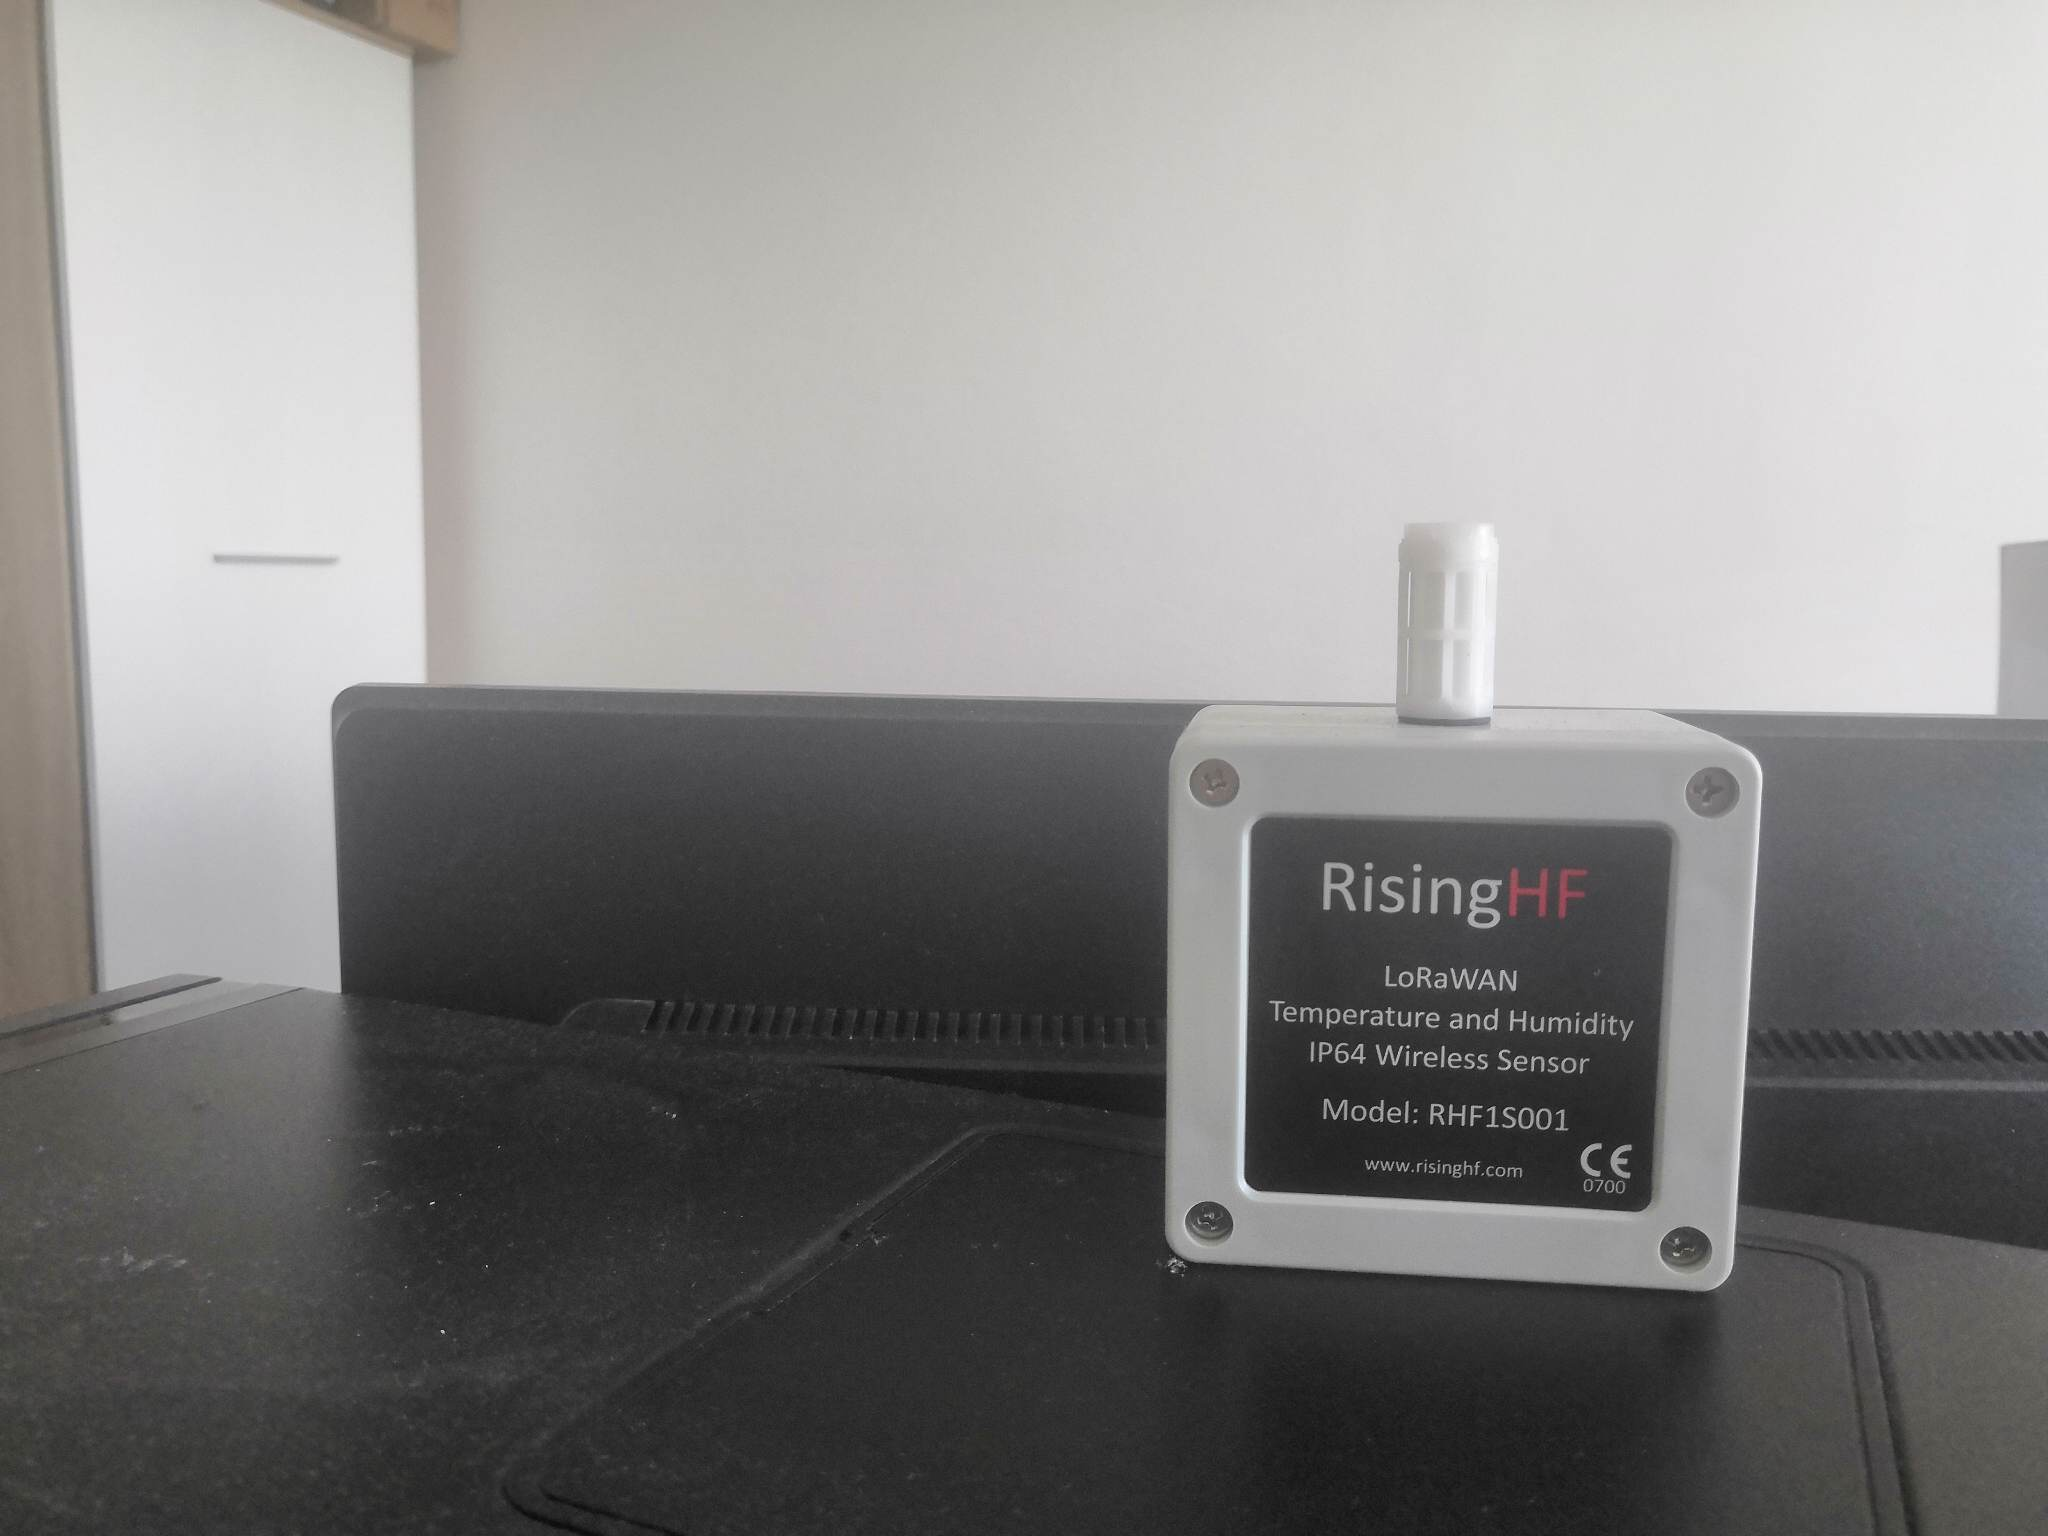
\includegraphics[width=\textwidth]{obrazky-figures/dev_picture_2.jpg}
    \end{subfigure}
    \caption{Zariadenia monitorujúce a ovládajúce teplotu miestnosti.}
    \label{fig:test_device}
\end{figure}

\begin{figure}[H]
    \centering
    \begin{subfigure}[b]{\textwidth}
        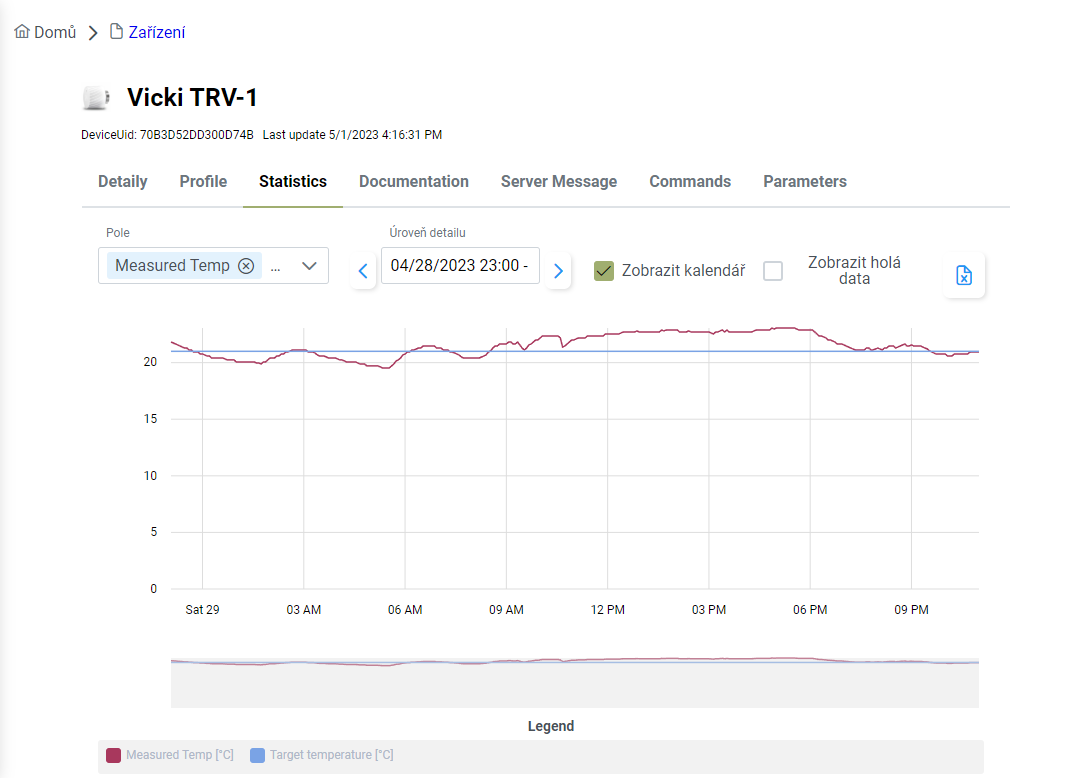
\includegraphics[width=\textwidth]{obrazky-figures/iTempStatisticTemp.png}
    \end{subfigure}
    \begin{subfigure}[b]{\textwidth}
        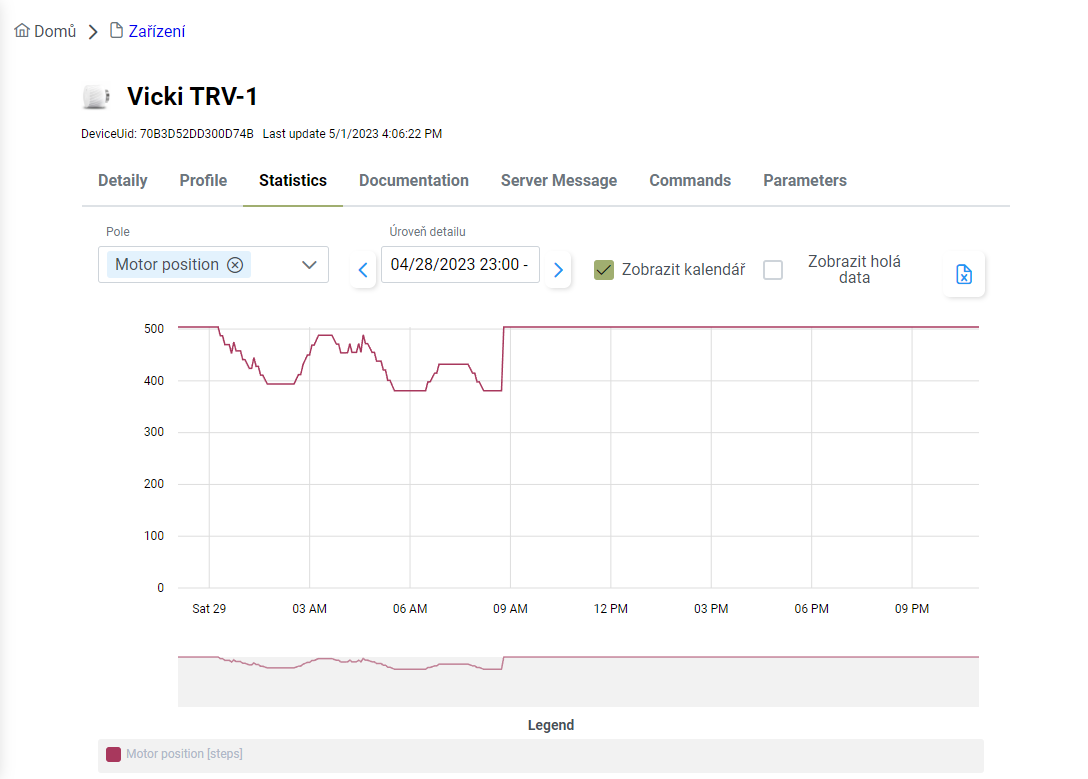
\includegraphics[width=\textwidth]{obrazky-figures/iTempStatisticPosition.png}
    \end{subfigure}
    \caption{Štatistiky z~aplikácie iTemp.}
    \label{fig:test_itempStat}
\end{figure}

\begin{figure}[H]
    \centering
    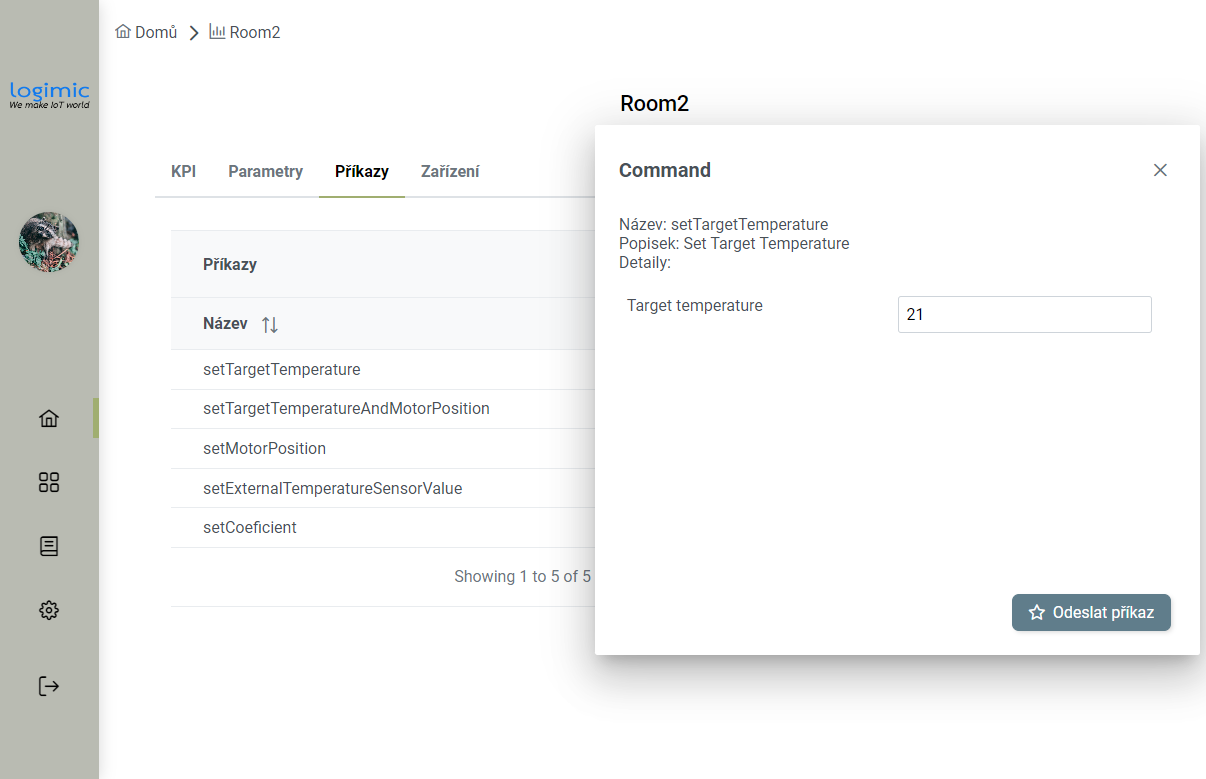
\includegraphics[width=0.9\textwidth]{obrazky-figures/setTarget.png}
    \caption{Nastavenie požadovanej teploty.}
    \label{fig:test_setTarget}
\end{figure}



\begin{figure}[H]
    \centering
    \includesvg[inkscapelatex=false,width=0.9\textwidth]{obrazky-figures/statisticGraph.svg}
    \caption{Graf vývoja teplôt a pozície motora v~čase s~chybou.}
    \label{fig:statisticGraph}
\end{figure}

\begin{figure}[H]
    \centering
    \includesvg[inkscapelatex=false,width=\textwidth]{obrazky-figures/statisticGraph01.svg}
    \caption{Graf vývoja teplôt a pozície motora v~čase.}
    \label{fig:statisticGraph01}
\end{figure}
  \chapter{Záver}\label{zaver}
Cieľom tejto bakalárskej práce bolo navrhnúť a implementovať systém regulácie ústredného kúrenia so zameraním na reguláciu jednotlivých miestností. 
Tento systém mal byť diaľkovo ovládateľný platformou Logimic Smart City a mal by automaticky regulovať vytápanie adaptívnym spôsobom. 
Tento spôsob by mal prinášať značné úspory do domácností, ktoré by boli takýmto systémom vybavené. 
Toto riešenie by sa malo oproti existujúcim riešeniam líšiť hlavne tým, že si do systému zadáme požadovanú teplotu miestnosti a systém bude ovládať výhrevné telesá aby požadovanú teplotu miestnosti docielil a udržal.

V rámci teoretickej části som si musel riadne naštudovať problematiku kúrenia a IoT. Nakoľko obe témy sú dosť robustné a pre mňa boli úplne nové, bol ich prieskumu a samoštúdiu venovaný značný čas. Poznatkami z kapitoly problematika kúrenia, dotazníkom, konzultáciou s firmou Virtuálny správca budov a hlavne konzultáciami s firmou Logimic som vyvodil požiadavky na inteligentné ovládanie kúrenia. Na základe toho som navrhol modul ovládania kúrenia pre existujúcu aplikáciu iTemp. Úpravy dashboardu neboli nutné, nakoľko táto aplikácia mala všetky potrebné ovládacie a zobrazovacie prvky. Spomínaný modul som implementoval a nasadil do ostrého riešenia aplikácie iTemp.
Túto implementáciu som následne testoval jak v realnom prostredí, tak aj v simulácii, v ktorej som aj skúšal rôzne spôsoby a modeli regulácie.

Tento systém je realne použiteľný a momentálne ovláda jednu konkrétnu miestnosť. V nej dosahuje dobrých výsledkov a udržiava požadovanú teplotu. Ďalej by bolo možné do systému zaviesť mnoho ďalšich funkcií, ktoré aj vyžadovali potencionálny zákazníci v dotazníku. Jedná sa napríklad o detekciu otvoreného okna, denné, týždenné a iné programy. Prípadne by bolo možné vylepšiť algoritmus o predikciu budúcnosti pre ešte lepšie a presnejšie ovládanie kúrenia.

  
  % Kompilace po částech (viz výše, nutno odkomentovat)
  % Compilation piecewise (see above, it is necessary to uncomment it)
  %\subfile{projekt-01-uvod-introduction}
  % ...
  %\subfile{chapters/projekt-05-conclusion}


  % Pouzita literatura / Bibliography
  % ----------------------------------------------
\ifslovak
  \makeatletter
  \def\@openbib@code{\addcontentsline{toc}{chapter}{Literatúra}}
  \makeatother
  \bibliographystyle{bib-styles/Pysny/skplain}
\else
  \ifczech
    \makeatletter
    \def\@openbib@code{\addcontentsline{toc}{chapter}{Literatura}}
    \makeatother
    \bibliographystyle{bib-styles/Pysny/czplain}
  \else 
    \makeatletter
    \def\@openbib@code{\addcontentsline{toc}{chapter}{Bibliography}}
    \makeatother
    \bibliographystyle{bib-styles/Pysny/enplain}
  %  \bibliographystyle{alpha}
  \fi
\fi
  \begin{flushleft}
  \bibliography{content-literature}
  \end{flushleft}

  % vynechani stranky v oboustrannem rezimu
  % Skip the page in the two-sided mode
  \iftwoside
    \cleardoublepage
  \fi

  % Prilohy / Appendices
  % ---------------------------------------------
  \appendix
\ifczech
  \renewcommand{\appendixpagename}{Přílohy}
  \renewcommand{\appendixtocname}{Přílohy}
  \renewcommand{\appendixname}{Příloha}
\fi
\ifslovak
  \renewcommand{\appendixpagename}{Prílohy}
  \renewcommand{\appendixtocname}{Prílohy}
  \renewcommand{\appendixname}{Príloha}
\fi
%  \appendixpage

% vynechani stranky v oboustrannem rezimu
% Skip the page in the two-sided mode
%\iftwoside
%  \cleardoublepage
%\fi
  
\ifslovak
%  \section*{Zoznam príloh}
%  \addcontentsline{toc}{section}{Zoznam príloh}
\else
  \ifczech
%    \section*{Seznam příloh}
%    \addcontentsline{toc}{section}{Seznam příloh}
  \else
%    \section*{List of Appendices}
%    \addcontentsline{toc}{section}{List of Appendices}
  \fi
\fi
  \startcontents[chapters]
  \setlength{\parskip}{0pt} 
  % seznam příloh / list of appendices
  % \printcontents[chapters]{l}{0}{\setcounter{tocdepth}{2}}
  
  \ifODSAZ
    \setlength{\parskip}{0.5\bigskipamount}
  \else
    \setlength{\parskip}{0pt}
  \fi
  
  % vynechani stranky v oboustrannem rezimu
  \iftwoside
    \cleardoublepage
  \fi
  
  % Přílohy / Appendices
  %\ifenglish
  %  \input{projekt-30-prilohy-appendices-en}
  %\else
  %  \input{projekt-30-prilohy-appendices}
  %\fi
  
  % Kompilace po částech (viz výše, nutno odkomentovat)
  % Compilation piecewise (see above, it is necessary to uncomment it)
  %\subfile{projekt-30-prilohy-appendices}
  
\end{document}
